\documentclass[xcolor=dvipsnames,10pt,aspectratio=169]{beamer}
%\usetheme[hideallsubsections]{Hannover}
%\usetheme[width=1.9cm]{Hannover} % plenty of themes to pick from
%\usetheme{Fredericksburg}
\usefonttheme[onlymath]{serif}
\graphicspath{{../../images/}}
\usepackage[utf8]{inputenc}
\usepackage[T1]{fontenc}
\usepackage{caption}
\usepackage{amsmath}
\usepackage{amsfonts}
\usepackage{amssymb}
\usepackage{braket}
\usepackage{bm}
\usepackage{textpos}
\usepackage{multicol}
\usepackage{graphicx,hyperref,url}
\usepackage{tikz}
\usepackage{verbatim}
\usepackage{pgfplots}
\usepackage{color}
\usetikzlibrary{arrows,decorations.pathmorphing,shapes}
\usecolortheme{crane} % plenty of color themes to pick from
\useinnertheme{rectangles}

\let\olditemize\itemize \renewcommand{\itemize}{\olditemize\itemsep5pt}

\definecolor{UBCgreen}{RGB}{30, 77, 43} % UBC Blue (primary)
\definecolor{UBCgold}{RGB}{200, 195, 114} % UBC Grey (secondary)


\setbeamercolor{palette primary}{bg=UBCgreen,fg=white}
\setbeamercolor{palette secondary}{bg=UBCgreen,fg=white}
\setbeamercolor{palette tertiary}{bg=UBCgreen,fg=white}
\setbeamercolor{palette quaternary}{bg=UBCgreen,fg=white}
\setbeamercolor{palette sidebar primary}{fg=black,bg=UBCgold}
\setbeamercolor{palette sidebar secondary}{fg=black,bg=UBCgold}
\setbeamercolor{palette sidebar tertiary}{fg=black,bg=UBCgold}
\setbeamercolor{palette sidebar quaternary}{fg=black,bg=UBCgold}
\setbeamercolor{structure}{fg=UBCgreen} % itemize, enumerate, etc
\setbeamercolor{section in toc}{fg=UBCgreen} % TOC sections
\setbeamercolor{subsection in head/foot}{bg=UBCgold,fg=white}
\setbeamercolor{section in sidebar}{fg=UBCgreen}
\setbeamercolor{section in sidebar}{fg=UBCgreen}
\setbeamerfont{section in sidebar}{size=\small}
\setbeamerfont{subsection in sidebar}{size=\scriptsize}
\setbeamerfont{title in sidebar}{size=\tiny}
\setbeamerfont{author in sidebar}{size=\tiny}
\setbeamertemplate{page number in head/foot}[appendixframenumber]
\setbeamertemplate{navigation symbols}{\footnotesize\usebeamertemplate{page number in head/foot}}
\setbeamertemplate{frametitle}[default][left,colsep=-4bp,rounded=false]
\setbeamertemplate{section in toc}[bullets]

\addtobeamertemplate{title page}{}{%
    \begin{textblock*}{100mm}(0.445\textwidth,-21.45em)
      
\includegraphics[width=1.35cm]{./figures/CSU-Ram-357-617.png}
    \end{textblock*}
    \begin{textblock*}{85em}(-1.0em,-12em)
      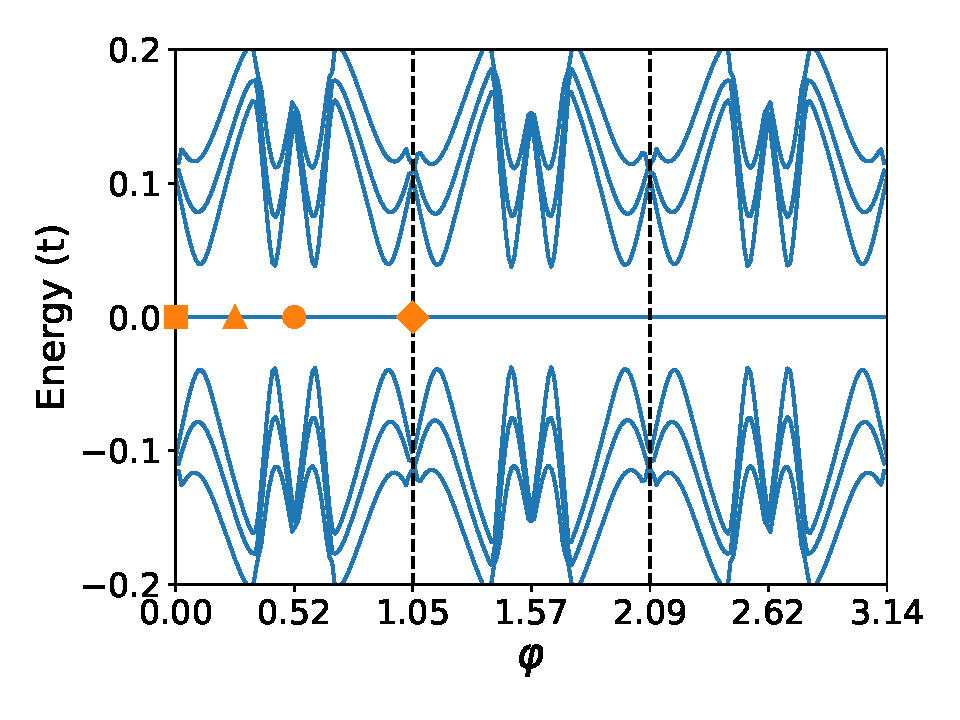
\includegraphics[width=0.18\textwidth]{./figures/spectral-flow-rotation-constant-vector-nr-50-w-1-mu-1_1.pdf}
    \end{textblock*}
    \begin{textblock*}{75em}(26.0em,-12em)
      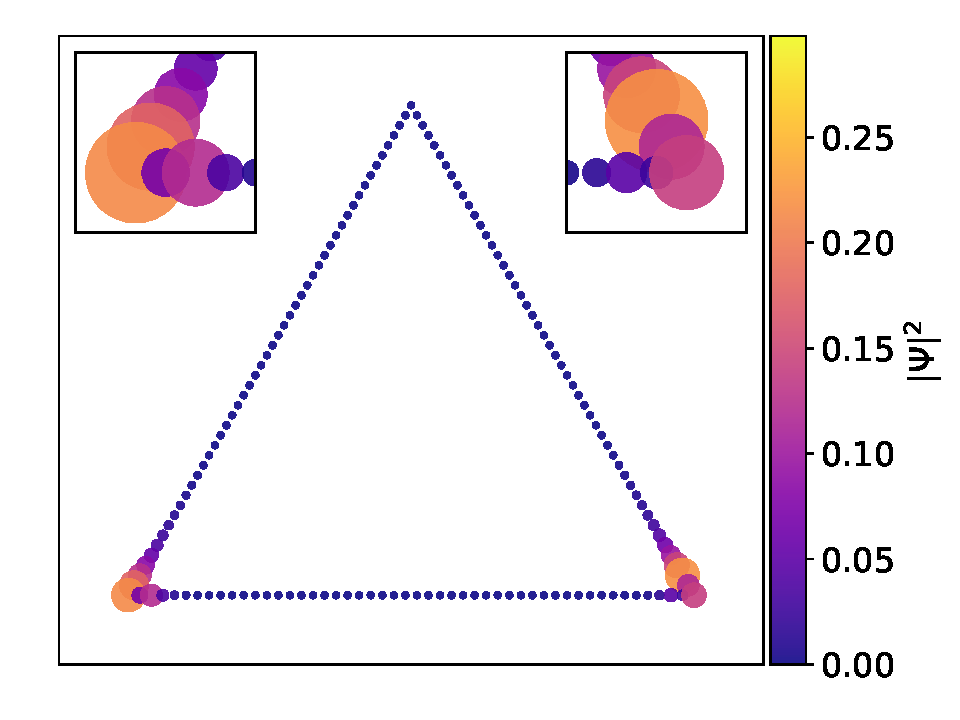
\includegraphics[width=0.19\textwidth]{./figures/GS-T-Square.pdf}
    \end{textblock*}
    \begin{textblock*}{100em}(-2.5em,1.8em)
      \tiny Built in \LaTeX
    \end{textblock*}
}

\addtobeamertemplate{frametitle}{}{%
    \begin{textblock*}{100mm}(0.95\textwidth,-0.95cm)
      
\includegraphics[width=0.925cm]{./figures/CSU-Ram-357-617.png}
    \end{textblock*}
}
\useoutertheme[subsection=false]{miniframes}
\makeatletter
\newcommand\letbeamertemplate[2]{%
  \csletcs{beamer@@tmpl@#1}{beamer@@tmpl@#2}%
}
%\setbeamertemplate{sidebar canvas \beamer@sidebarside}%
                  %[vertical shading][top=UBCgold,bottom=UBCgold]
\letbeamertemplate{footline}{headline}
% Then, reset `headline`
\setbeamertemplate{headline}[default]
\makeatother

%\addtobeamertemplate{sidebar left}{}{
%  \hspace{0.3cm}
%  \vspace{0.2cm}
%  
\includegraphics[align = l, width = 1cm]{./figures/CSU-Ram-357-617.png}
%}

\setbeamertemplate{section in toc}{\hspace*{0em}\inserttocsection}
\setbeamertemplate{subsection in toc}{\hspace*{2em}\inserttocsubsection}

\let\oldhat\hat
\let\op\hat
\renewcommand{\hat}[1]{\oldhat{\mathbf{#1}}}
\renewcommand{\vec}[1]{\mathbf{#1}}

\newcommand{\ham}{\mathcal{H}}
\newcommand{\ke}{k_{\epsilon}}
\newcommand{\kpm}{k_{\pm}}
\newcommand{\sx}{\sigma_x}
\newcommand{\sy}{\sigma_y}
\newcommand{\sz}{\sigma_z}
\newcommand{\so}{\sigma_0}
\newcommand{\cc}{c^{\dagger}}
\newcommand{\de}{\Delta}

\newcommand{\TT}{Emergent Topological Phenomena in Low-Dimensional Systems Induced by Gauge Potentials}
\newcommand{\ST}{Emergent topological phenomena in low-dimensional systems induced by gauge potentials}
\newcommand{\BD}{Background}
\newcommand{\MO}{Motivation}
\newcommand{\FO}{Formulation}
\newcommand{\RE}{Results}
\newcommand{\CO}{Summary}

\title[\ST]{\TT}
\subtitle{}
\author[Aidan Winblad]{Aidan Winblad \small \and\\ Hua Chen}
\institute{Department of Physics \and\\ Colorado State University}
\date{\small March 14, 2025}

\begin{document}
  \begin{frame}
  \titlepage
  \end{frame}

  \begin{frame}{Presentation objectives}

    Part I: Topological superconducting triangular islands
    \begin{itemize}
      \item Construct a new platform for topological quantum logic gates via:
        \begin{itemize}
          \item Triangular geometry
          \item Applied gauge potentials
        \end{itemize}
    \end{itemize}
    \vspace{5mm}
    Part II: Floquet quantum Hall effect
    \begin{itemize}
      \item Induce quantum Hall effect with inhomogeneous, circularly polarized light via:
        \begin{itemize}
          \item Floquet theorem
          \item High-frequency approximation
        \end{itemize}
    \end{itemize}
  \end{frame}

  \section{I: \BD}

  \begin{frame}
  \frametitle{Part I: Topological superconducting triangular islands outline}
    \begin{itemize}
      \item \BD:
        \begin{itemize}
          \footnotesize
          \item What does topology offer for quantum computing
          \item What are Majorana fermions and where to find them
          \item Kitaev chain and Majorana number
        \end{itemize}
      \item \MO:
        \begin{itemize}
          \footnotesize
          \item Braiding and topological quantum computing
          \item T-junctions to triangular structures
        \end{itemize}
      \item \RE:
        \begin{itemize}
          \footnotesize
          \item Minimal Kitaev triangle
          \item Hollow triangular islands
          \item Minimal braiding example
        \end{itemize}
      \item \CO
      %\item Additional Research
      %  \begin{itemize}
      %    \footnotesize
      %    \item Floquet quantum Hall effect
      %  \end{itemize}
    \end{itemize}
  \end{frame}

  \begin{frame}{What does topology offer for quantum computing?}
    \begin{itemize}
      \visible<1->{
      \item Quantum computers have two prominent ``local'' errors (noise, perturbations).
      %\item[]
      \begin{itemize}
        \item Classical error: flips a qubit from empty to occupied, $|0\rangle \rightarrow |1\rangle$, or vice versa.
        %\item[]
        \item Phase error: changes the sign of an occupied qubit, $|1\rangle \rightarrow -|1\rangle$.
        %\item[]
        \item Normal qubits have various means for reducing error and achieving fault-tolerance.
      \end{itemize}
      }
      \visible<2->{
      %\item[]

      \item Topological qubits have fault-tolerance baked in.
      \begin{itemize}
        \item Their qubit information is stored ``non-locally'', making the above errors unlikely to occur.
        \item What system allows for topological qubits?
      \end{itemize}
      }
    \end{itemize}

    \vspace{1cm}
    \centering
    \visible<3>{
    \textbf{Majorana fermions are candidates for building topological quantum computers.}}

  \end{frame}

  \begin{frame}{What are Majorana fermions?}
    \begin{columns}
      \column{0.5\textwidth}
      \centering
      \begin{tikzpicture}[>=stealth',  pos=.8,photon/.style={decorate,decoration={snake,post length=1mm}}
]
        \visible<1->{\node[inner sep=0pt] (figure) at (-1.5,0)
        {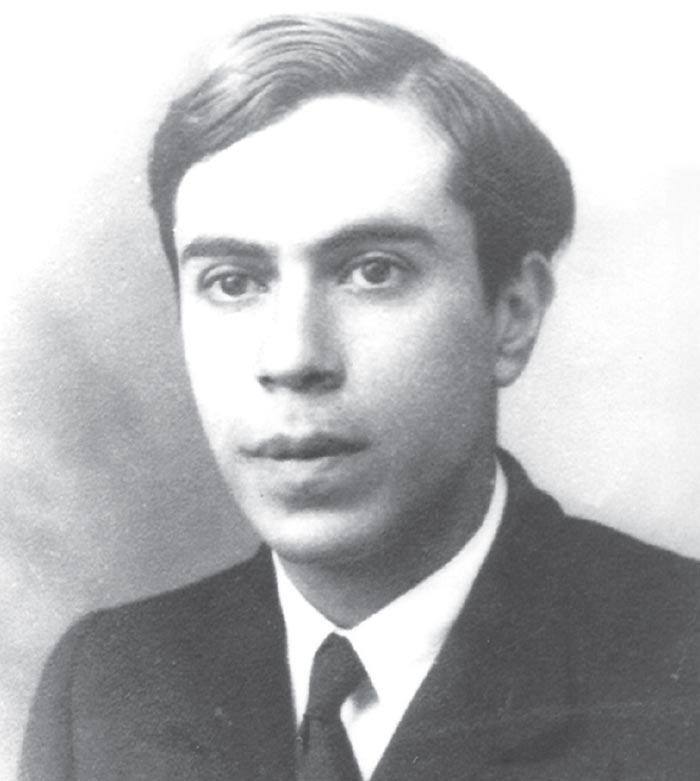
\includegraphics[height=0.3\textheight]{./figures/Ettore_Majorana.jpg}};}
        \visible<1->{\node[inner sep=0pt] (Ettore) at (-1.5,1.55) {\small Ettore Majorana};}
        %\visible<2>{\node[inner sep=0pt] (arrow) at (0,0.0) {$\rightarrow\ \leftarrow$};}
        %\visible<2>{\node[inner sep=0pt] (figure) at (1.5,0)
        %{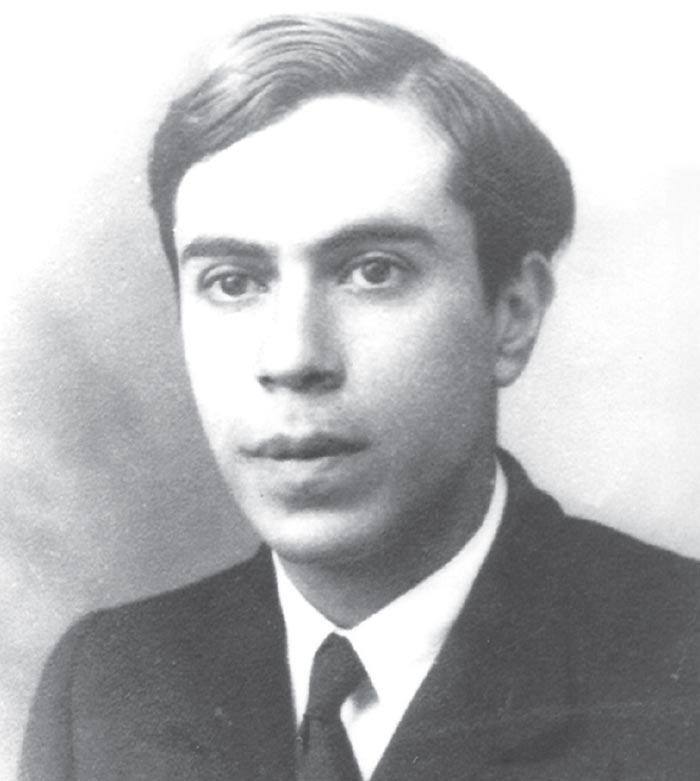
\includegraphics[height=0.3\textheight]{./figures/Ettore_Majorana.jpg}};}
        %\visible<2>{\node[inner sep=0pt] (Ettore) at (1.5,1.55) {\small Doppelganger};}

        %\visible<3>{
        %\draw[->,photon] (0,0) -- node[above left] {} (30:2);
        %\draw[->,photon] (0,0) -- node[below left] {} (150:2);}

      \end{tikzpicture}

      \vspace{1em}
      \begin{tikzpicture}
        \node[inner sep=0pt] (figure) at (0,0)
        {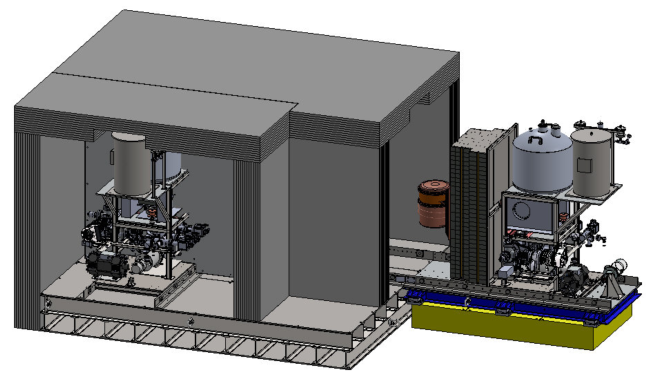
\includegraphics[height=0.3\textheight]{./figures/majorana-experiment.png}};
        \node[inner sep=0pt] (reference) at (0,-1.4) {\small MAJORANA project};
      %\node[inner sep=0pt] (reference) at (0,-1.8) {\small neutrinoless double beta (0$\nu\beta\beta$) decay};
      \end{tikzpicture}

      \column{0.5\textwidth}
      \begin{itemize}
        \setlength\itemsep{0pt}
        \item Fermions
          \begin{itemize}
            \item Fermi-Dirac statistics
            \item Pauli exclusion principle
            \item Half-odd-integer spin
          \end{itemize}
      \end{itemize}

      \begin{itemize}
        \setlength\itemsep{0pt}
        \item Majorana Fermions (MFs)
        \begin{itemize}
            \item Particle $=$ Antiparticle
            \item Neutral, Massive
            \item Negative results for Majorana particles as elementary particles
        \end{itemize}
      \end{itemize}

    \end{columns}

  \end{frame}

  \begin{frame}{Where to find Majorana fermions?}
    \begin{columns}
      \column{0.5\textwidth}
      \begin{itemize}
        \item Superconductors (SCs)
          \begin{itemize}
            \item Cooper pairs
            \begin{itemize}
              \item Electron-phonon interaction pairs two electrons with opposite spin and momenta.
            \end{itemize}
            \pause
            \item Bogoliubov quasiparticles
            \begin{itemize}
              \item Excitation, pairs an electron to a hole with opposite momenta.
              \item[] \[ H_{BdG} = \begin{bmatrix} \epsilon(k) & \de(k) \\ \de^\ast(k) & -\epsilon(-k) \end{bmatrix} \]
              \item Zero-energy excitations in non-tivial \textit{p}-wave SC may be MFs.
              \item Come in pairs.
            \end{itemize}
          \end{itemize}
      \end{itemize}

      \column{0.5\textwidth}
      \begin{figure}
        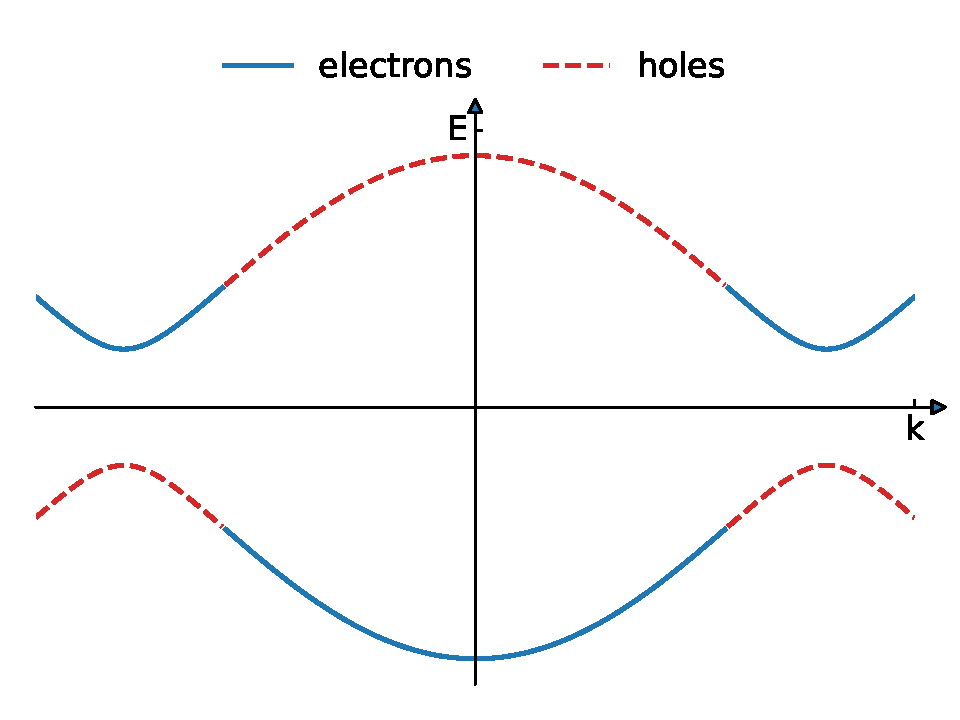
\includegraphics[width=0.90\textwidth]{./figures/p-wave-mu-p1_25.pdf}
      \end{figure}

    \end{columns}

  \end{frame}

  \begin{frame}{Kitaev chain - 1D \textit{p}-wave superconducting wire}
    \centering
    \begin{tikzpicture}
      \node[inner sep=0pt] (f2) at (0,0) {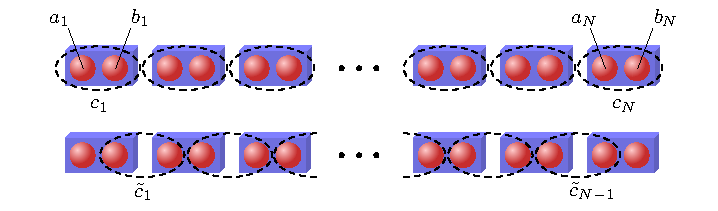
\includegraphics[width=0.9\textwidth]{./figures/kitaev-chain.pdf}};
      \visible<1>{\draw[draw=white, fill=white] (-5.5,0.5) rectangle (5.8,-3.5);}
      \visible<2>{\draw[draw=white, fill=white] (-1.5,-2.7) rectangle (1.5,-3.5);}
      \visible<3>{\draw[line width=2pt, draw=UBCgold] (-1.5,-2.7) rectangle (1.5,-3.5);}
    \end{tikzpicture}
  \end{frame}

  \begin{frame}{Band gap and topological phase}
    \begin{tikzpicture}
      \visible<1->{
      \node[inner sep=0pt] (tp) at (-4.6,0)
      {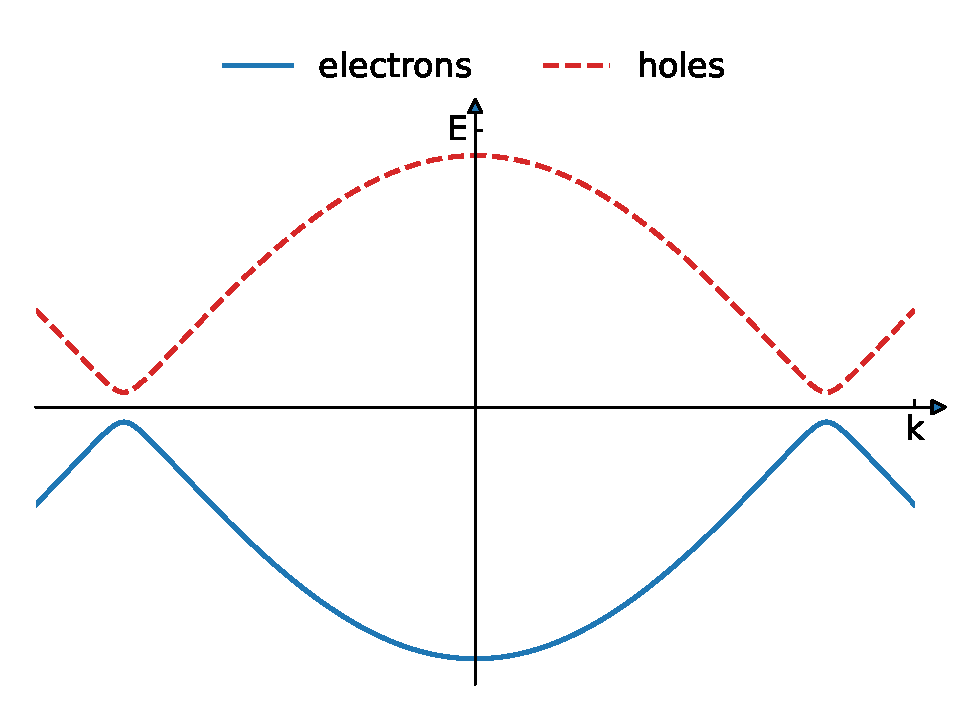
\includegraphics[width=0.33\textwidth]{./figures/p-wave-mu-p2_25.pdf}};
      \node[inner sep=0pt] (tp) at (-4.6,-2.0) {\footnotesize $\mu=2.25t$};
      \node[inner sep=0pt] (Mtp) at (-4.6,-2.5) {\footnotesize $\mathcal{M}=1$};
      \node[inner sep=0pt] (tp) at (-4.6,-3.0) {\footnotesize Trivial};
      }

      %\pause
      \visible<2->{
      \node[inner sep=0pt] (cp) at (0,0)
      {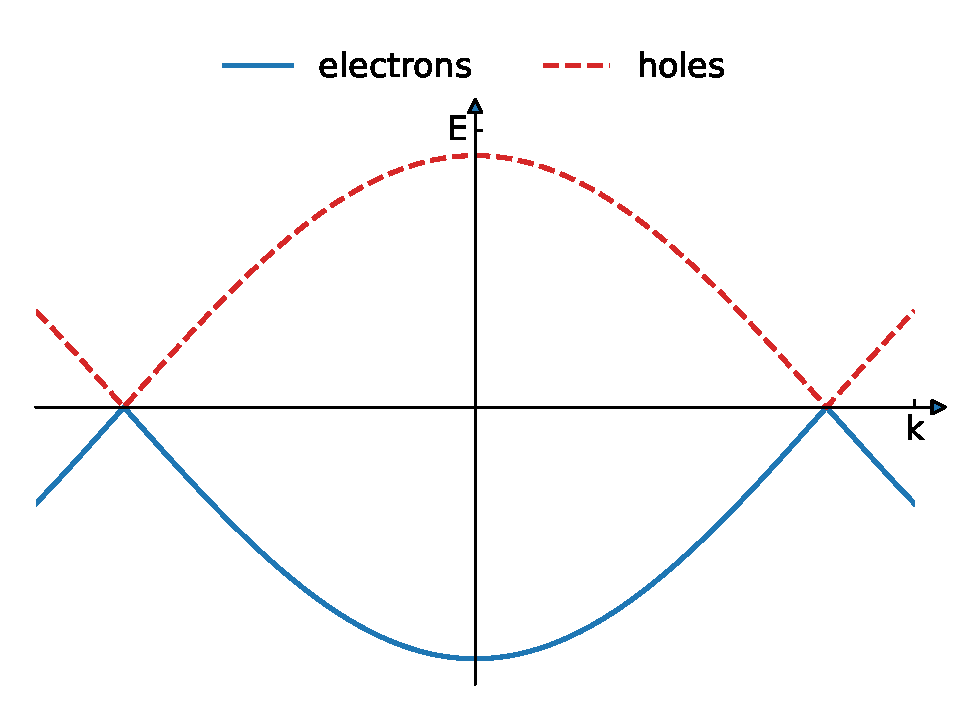
\includegraphics[width=0.33\textwidth]{./figures/p-wave-mu-p2_00.pdf}};
      \node[inner sep=0pt] (cp) at (0.0,-2.0) {\footnotesize $\mu_c=2t$};
      }

      %\pause
      \visible<3->{
      \node[inner sep=0pt] (ntp) at (4.6,0)
      {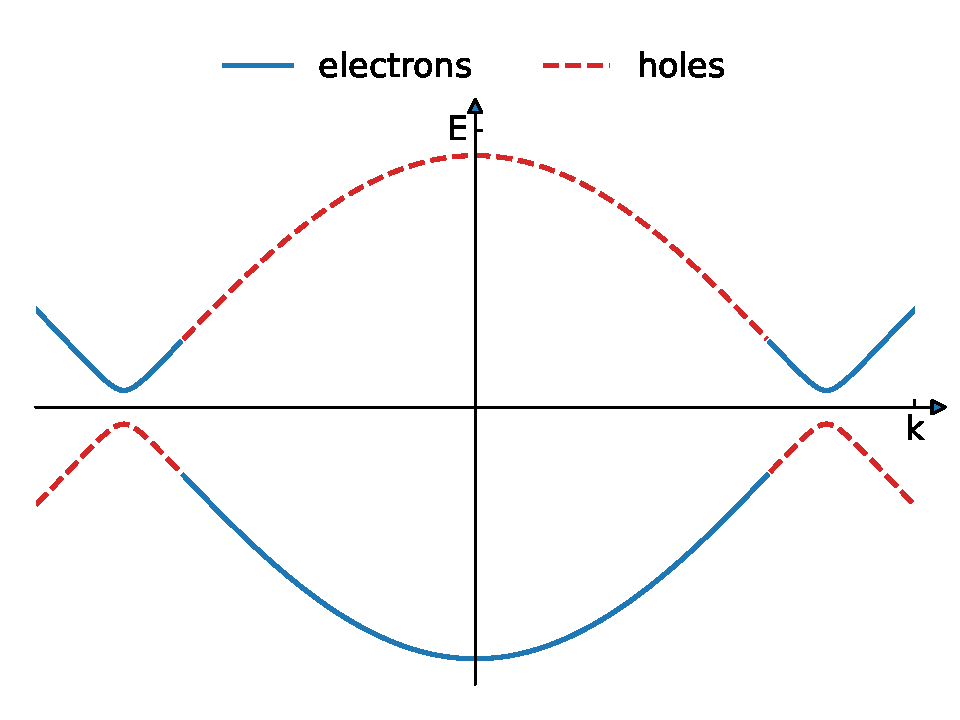
\includegraphics[width=0.33\textwidth]{./figures/p-wave-mu-p1_75.pdf}};
      \node[inner sep=0pt] (ntp) at (4.6,-2.0) {\footnotesize $\mu=1.75t$};
      \node[inner sep=0pt] (Mntp) at (4.6,-2.5) {\footnotesize $\mathcal{M}=-1$};
      \node[inner sep=0pt] (tp) at (4.6,-3.0) {\footnotesize Non-trivial};
      }

      %\pause
      \visible<4->{
      \node[inner sep=0pt] (ntp) at (0, -3.5) {\small \underline{Non-trivial phase}};
      \node[inner sep=0pt] (ntp) at (0, -4.0) {\small larger band gap $\rightarrow$ more robust against local errors $\rightarrow$ stronger topological protection};
    }

    \end{tikzpicture}
  \end{frame}

  \begin{frame}{Majorana number \& bulk-edge correspondence}
    %Majorana number topological invariant 1D SC

    \small
    Transform to Majorana basis
    \begin{equation*}
      A = -i U \ham U^{\dagger}
    \end{equation*}
    Majorana number
    \begin{equation*}
      \mathcal{M} = \text{sgn}[\text{Pf}(A)]
    \end{equation*}

    %Particle-hole symmetry in momentum-space allows
    %\begin{equation}
    %  \mathcal{M} =
    %  \begin{cases}
    %    \text{sgn} [\text{Pf} (A_{k=0}) \text{Pf} (A_{k=\pi})], &\text{if L is even}      , \\
    %    \text{sgn} [\text{Pf} (A_{k=0})], &\text{if L is odd},
    %  \end{cases}
    %\end{equation}

    \begin{itemize}
      \item If $|\mu| > 2t$, $\mathcal{M} = +1$, trivial topology
      \item If $|\mu| < 2t$, $\mathcal{M} = -1$, non-trivial topology
    \end{itemize}

    \begin{figure}
      \visible<2->{
      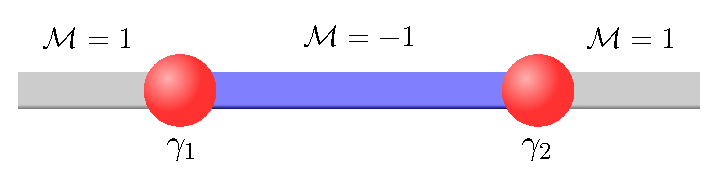
\includegraphics[width = 0.6\textwidth]{./figures/bulk-edge.pdf}
      }
    \end{figure}

    \centering
    \visible<3>{
    \textbf{Warning! There are no \textit{p}-wave SCs currently, but we can build effective \textit{p}-wave SCs!}
    }

  \end{frame}

  \begin{frame}{Experimental evidence of Majorana fermions I}
    \begin{columns}
      \column{0.5\textwidth}
      \centering
      \begin{tikzpicture}
        \node[inner sep=0pt] (figure) at (0,0)
        {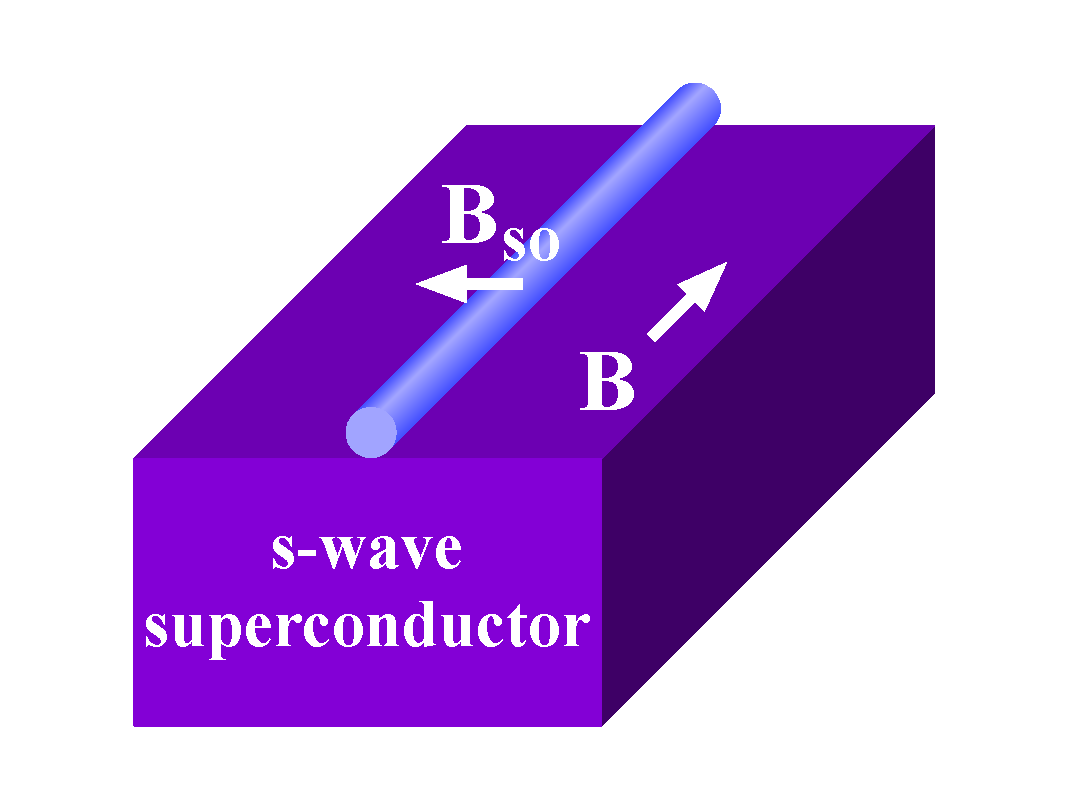
\includegraphics[height=0.40\textheight]{./figures/swave-superconductor.pdf}};
      \end{tikzpicture}
      \begin{tikzpicture}
        \node[inner sep=0pt] (figure) at (0,0)
        {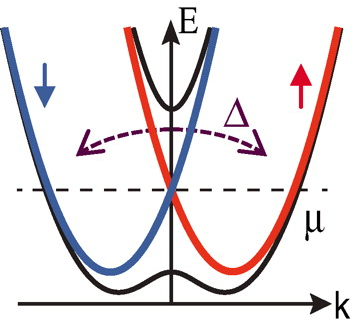
\includegraphics[height=0.40\textheight]{./figures/Mourik-dispersion.jpeg}};
      \end{tikzpicture}
      \vspace{40pt}
      \column{0.5\textwidth}
      \begin{tikzpicture}
        \node[inner sep=0pt] (figure) at (0,0)
        {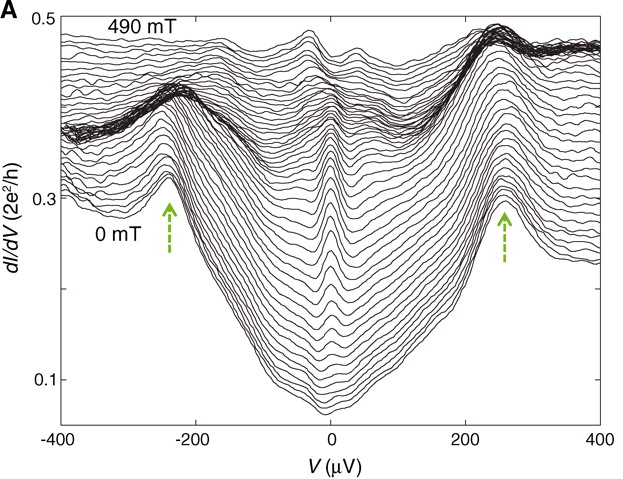
\includegraphics[width=1.00\textwidth]{./figures/Mourik-didv-curve.png}};
        \draw[line width = 2pt, draw=red] (0.23, 0.12) ellipse (0.5 and 2.5);
        \node[inner sep=0pt] (reference) at (0.0,-3) {\footnotesize Mourik et al., \textit{Science} \textbf{336}, 1003 (2012)};
      \end{tikzpicture}
    \end{columns}
  \end{frame}

  \begin{frame}{Experimental evidence of Majorana fermions II}
    \begin{tikzpicture}
      \node[inner sep=0pt] (figure) at (-3.6,0)
      {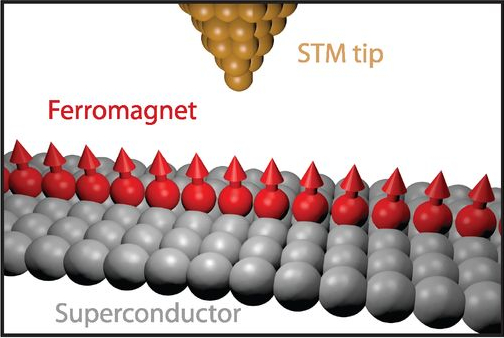
\includegraphics[width=0.5\textwidth]{./figures/Nadj-Perge-setup.png}};
      \node[inner sep=0pt] (figure) at (3.6,0)
      {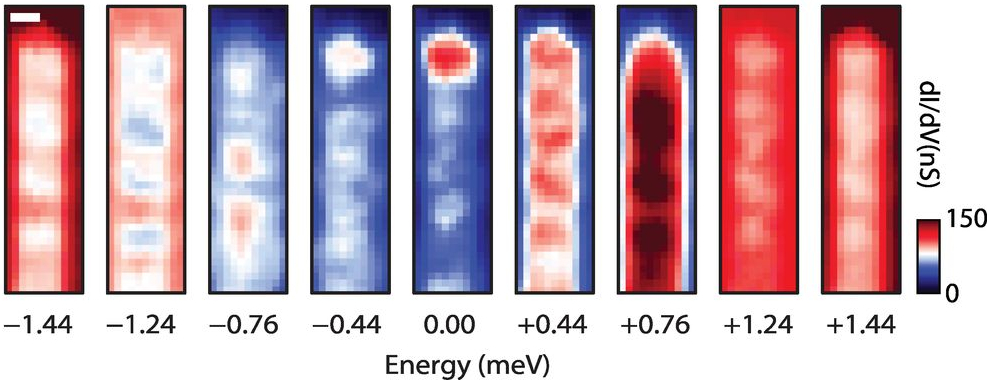
\includegraphics[width=0.5\textwidth]{./figures/Nadj-Perge-results.png}};
      \draw[line width=2pt, draw=red] (2.95,1.40) rectangle (3.67, -1.10);
      \node[inner sep=0pt] (reference) at (3.60,-1.75) {\footnotesize Nadj-Perge et al., \textit{Science} \textbf{346}, 602 (2014)};
    \end{tikzpicture}
  \end{frame}

  \begin{frame}{Experimental evidence of Majorana fermions III}
    \centering
    \begin{tikzpicture}
      \node[inner sep=0pt] (figure) at (0,0)
      {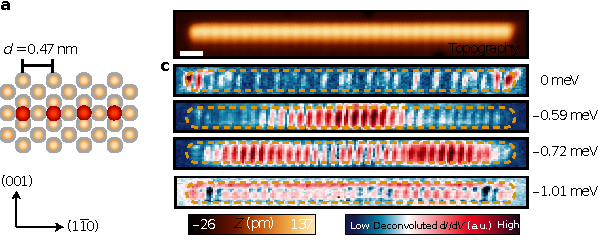
\includegraphics[width=\textwidth]{./figures/Schneider-results.pdf}};
      \node[inner sep=0pt] (reference) at (0,-3.00) {\footnotesize Mn atoms (red spheres) on top of superconducting Nb (brown spheres).};
      \draw[line width=2pt, draw=red] (-3.0,1.38) rectangle (6.7, 0.50);
      \node[inner sep=0pt] (reference) at (0,-3.40) {\footnotesize Schneider et al., \textit{Nature Nanotechnology} \textbf{17}, 384 (2022)};
    \end{tikzpicture}

    \centering
    \visible<2>{
      \textbf{Zero-energy states could be Andreev bound states. ``Braiding'' can distinguish them.}
    }
  \end{frame}

  \section{I: \MO}

  \begin{frame}
    \frametitle{What makes Majorana fermions so cool?}
    \begin{columns}
      \column{0.6\textwidth}

        \begin{itemize}
          \visible<1->{\item 2D \textit{p}-wave (triplet pairing) SC exhibit half-quantum vortices.}
          \vspace{1em}
          \visible<2->{\item  MF state accumulate $e^{i\theta/2}$ phase.}
          \vspace{1em}
          \visible<3->{
          \item Braiding demonstrates non-Abelian statistics i.e.\ $A*B \neq B*A$,
          \begin{itemize}
            \item[\rightarrow] Allows for a universal quantum computer.
          \end{itemize}
          }
          \vspace{1em}
          \visible<4->{\item Combine with MFs topological protection,
          \begin{itemize}
            \item[\rightarrow] Topological quantum computer.
            \item[\rightarrow] Benefits: fewer repeated operations compared to normal qubits.
          \end{itemize}
          }
        \end{itemize}
      \column{0.4\textwidth}

      \visible<2->{
      \begin{align*}
        \gamma_1 &\rightarrow -\gamma_2 \\
        \gamma_2 &\rightarrow \gamma_1
      \end{align*}
      }
      \vspace{-5mm}

      \begin{tikzpicture}
        \visible<1>{
        \node[inner sep=0pt] (f1) at (0,0) {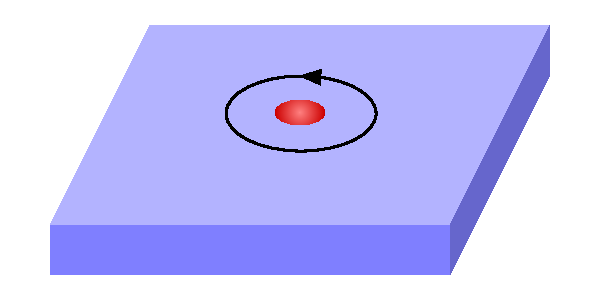
\includegraphics[width=\textwidth]{./figures/vortex.pdf}};
        }

        \visible<2->{
        \node[inner sep=0pt] (f1) at (0,0) {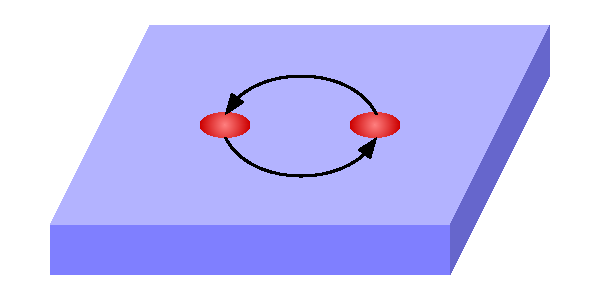
\includegraphics[width=\textwidth]{./figures/braiding.pdf}};
        \node[inner sep=0pt] (g1) at (-1.15,0.25) {$\gamma_1$};
        \node[inner sep=0pt] (g2) at (1.15,0.25) {$\gamma_2$};
        }
      \end{tikzpicture}
      \visible<3->{
      \begin{equation*}
        U_{12} = \exp\left(\pm\dfrac{\pi}{4} \gamma_1\gamma_2 \right)
      \end{equation*}
      }
    \end{columns}
  \end{frame}

  \begin{frame}{Braiding in a topological quantum computer}
    \vspace{-10mm}
    \begin{columns}
      \column{0.55\textwidth}
      \begin{figure}
        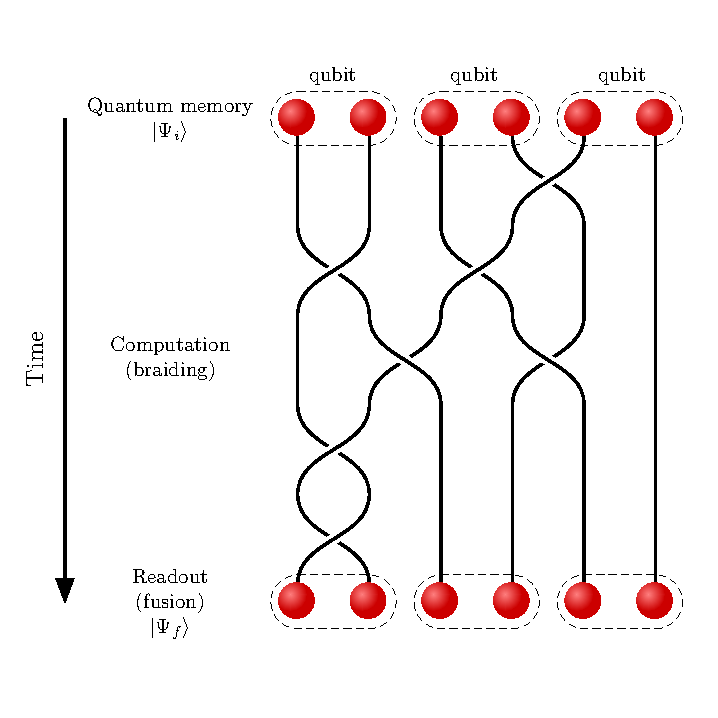
\includegraphics[height=1.0\textheight]{./figures/braid-network.pdf}
      \end{figure}
      \column{0.45\textwidth}
      \small
      Generalized braiding of two neighboring MFs
      \begin{align*}
        U_{nm} = \exp\left(\pm\dfrac{\pi}{4} \gamma_n\gamma_m \right) \\ \\
      \end{align*}
      Readout after braiding
      \begin{align*}
        |\Psi_f\rangle = U_{n'm'} \cdots U_{nm} |\Psi_i\rangle
      \end{align*}
    \end{columns}

  \end{frame}

  \begin{frame}{T-junction as a quantum logic gate}

    \begin{columns}
      \column{0.3\textwidth}
      \begin{figure}
        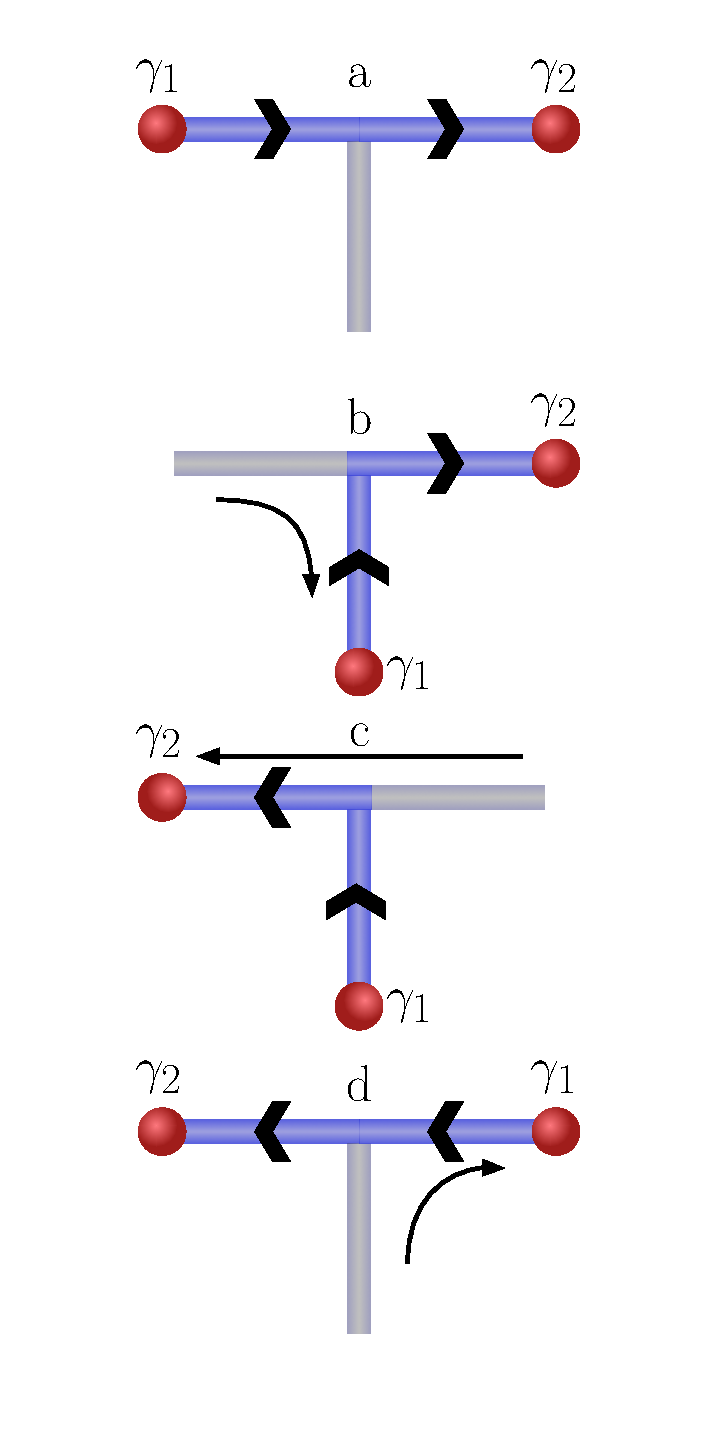
\includegraphics[height=0.85\textheight]{./figures/t-junction-braid.pdf}
      \end{figure}

      \column{0.7\textwidth}
      \small
      %\begin{equation}
      %  \ham_T = -\mu \sum_j \cc_j c_j - \sum_j t \cc_j c_{j+1} + |\de| e^{i\phi} c_j c_{j+1} + h.c.
      %\end{equation}
      %\begin{equation}
      %  c_j = e^{-i(\phi/2)}(\gamma_{j+1,1} + i \gamma_{j,2})/2
      %\end{equation}
      \begin{itemize}
        \small
        \item Take pairing term $|\de|e^{i\phi} c_j c_{j+1}$ such that the site indices:
        \item Increase moving $\rightarrow / \uparrow$ in the horizontal/vertical wires: $\phi=0$,
        \item Decrease moving $\leftarrow / \downarrow$ in the horizontal/vertical wires: $\phi=\pi$.
      \end{itemize}
      \centering

      \begin{tikzpicture}
        \node[inner sep=0pt] (figure) at (0,0)
        {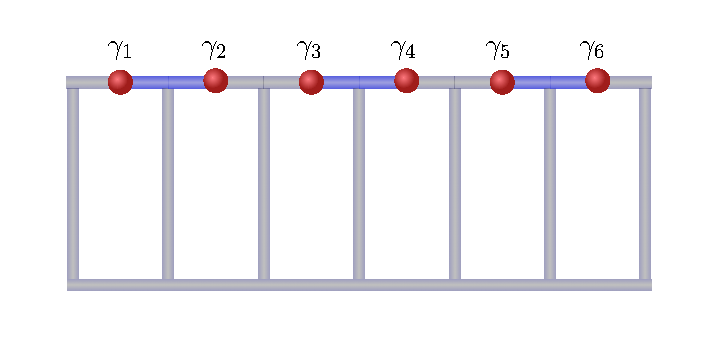
\includegraphics[width=0.75\textwidth]{./figures/ladder-junction.pdf}};
        \node[inner sep=0pt] (reference) at (0,-1.5) {\small Alicea et al., \textit{Nature Phys.} \textbf{7}, 412 (2011)}
      \end{tikzpicture}

      \visible<2>{
        \begin{itemize}
          \item[] \textbf{Difficult to build, manipulate, and read.}
          \item[] \textbf{Not a smooth connection between 1D and 2D SCs.}
        \end{itemize}
      }

    \end{columns}
  \end{frame}

  \begin{frame}
    \frametitle{Triangular structures for braiding}
    \begin{columns}

    \column{0.5\textwidth}
    \begin{itemize}
      \item T-junction $\rightarrow$ Triangle
      \item[] 3 endpoints $\rightarrow$ 3 vertices
      \visible<2->{\item Islands of three-fold rotational symmetry occur naturally in epitaxial growth on close-packed metal surfaces.}
      \visible<3>{\item In plane gauge potentials can break a triangle's 3-fold symmetry.}
      \visible<3>{\item Make a smoother connection between 1D and 2D superconductors.}
    \end{itemize}
    \newline

    \column{0.5\textwidth}
    \centering
    \begin{tikzpicture}
      \visible<2->{
      \node[inner sep=0pt] (figure) at (0,0)
      {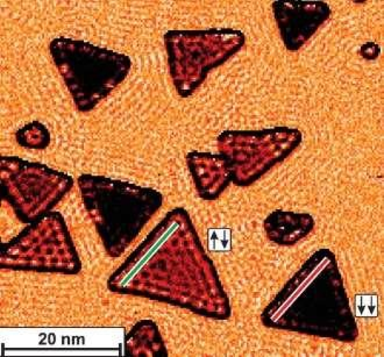
\includegraphics[height=0.7\textheight]{./figures/triangular-islands.pdf}};
      \node[inner sep=0pt] (caption) at (0,-3.2) {\scriptsize Triangular Co islands on Cu(111).};
      \node[inner sep=0pt] (reference) at (0,-3.6) {\small Pietzsch et al., \textit{PRL} \textbf{96}, 237203 (2006)};
      }
      \end{tikzpicture}
    \end{columns}

  \end{frame}

  \section{I: \RE}

  \begin{frame}{Two proposals}
    \begin{itemize}
      \item Exactly solvable minimal ``Kitaev Triangle''
        \begin{itemize}
          \item Three fermion sites compared to minimal four in T-junctions
          \item Three edges controlled by Peierls phase
        \end{itemize}
      %\item[]
      \pause
      \item Finite-size triangle with hollow interior
        \begin{itemize}
          %\item[]
          \item Uniform gauge potential
          %\item[]
          \item Bulk-edge correspondence
        \end{itemize}
    \end{itemize}
  \end{frame}

  \begin{frame}{Kitaev triangle}
    \small
    \begin{columns}
      \column{0.4\textwidth}
      \centering
      \begin{figure}
        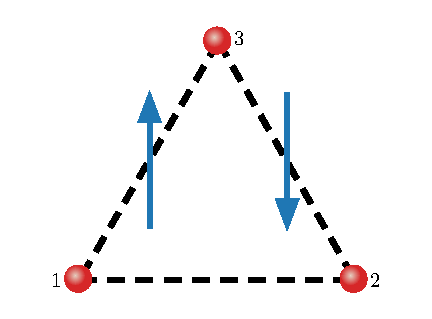
\includegraphics[width=1.25\textwidth]{./figures/3-point-triangle.pdf}
      \end{figure}

      \column{0.6\textwidth}
      \begin{align*}
        \vec{A} = \left[1-2\Theta(x) \right] \dfrac{2\pi}{3\sqrt{3}} \hat{y}
      \end{align*}
      \visible<2->{
      \begin{align*}
        \phi_{jl} = \frac{i e}{\hbar} \int_{r_j}^{r_l} \vec{A} \cdot d\vec{l}
      \end{align*}
      %\begin{align}
      %  \cc_j c_l &\rightarrow \cc_j c_l e^{i \phi_{jl}}
      %\end{align}
      \begin{align*} \label{eq: Peierls chain}
        \ham = \sum_{\langle j,l\rangle} (-t e^{i\phi_{jl}} \cc_j c_l + \de \cc_j\cc_l + h.c.) - \mu \cc_j c_j
      \end{align*}
      }

      \visible<3>{
      \centering
      \vspace{1em}
      In Kitaev limit, $t=\de\neq0$ and $\mu=0$,
      \begin{align*}
        (\phi_{12}, \phi_{23}, \phi_{31}) = (0, -\tfrac{\pi}{3}, -\tfrac{\pi}{3}) = \bm\phi_1
      \end{align*}
      MZMs localized at sites 1 and 2
    }
    \end{columns}
  \end{frame}

  \begin{frame}{Kitaev triangle braiding}
    \footnotesize
    A closed parameter path linearly interpolated between the following sets of $\phi_{jk}$:
    \begin{equation}
      (\phi_{12}, \phi_{23}, \phi_{31}) : \bm\phi_1 \rightarrow \bm\phi_2 \rightarrow \bm\phi_3 \rightarrow \bm\phi_1
    \end{equation}

    \begin{tikzpicture}
      \node[inner sep=0pt] (figure) at (-3.8,0.35)
      {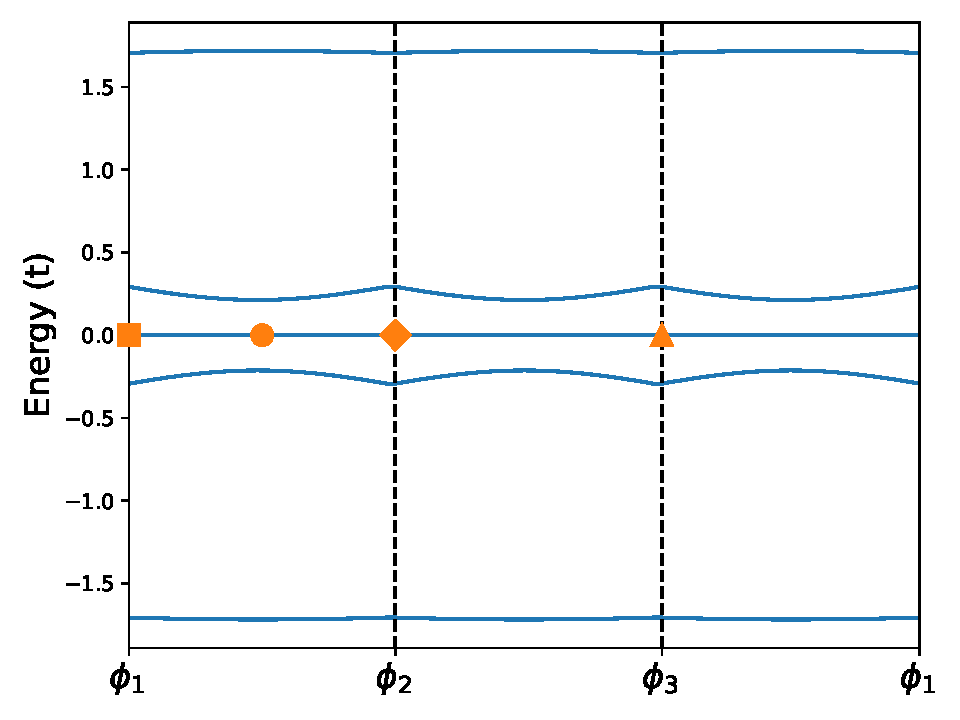
\includegraphics[width=0.5\textwidth]{./figures/3eigval.pdf}};
      \node[inner sep=0pt] (figure) at (3.8,0)
      {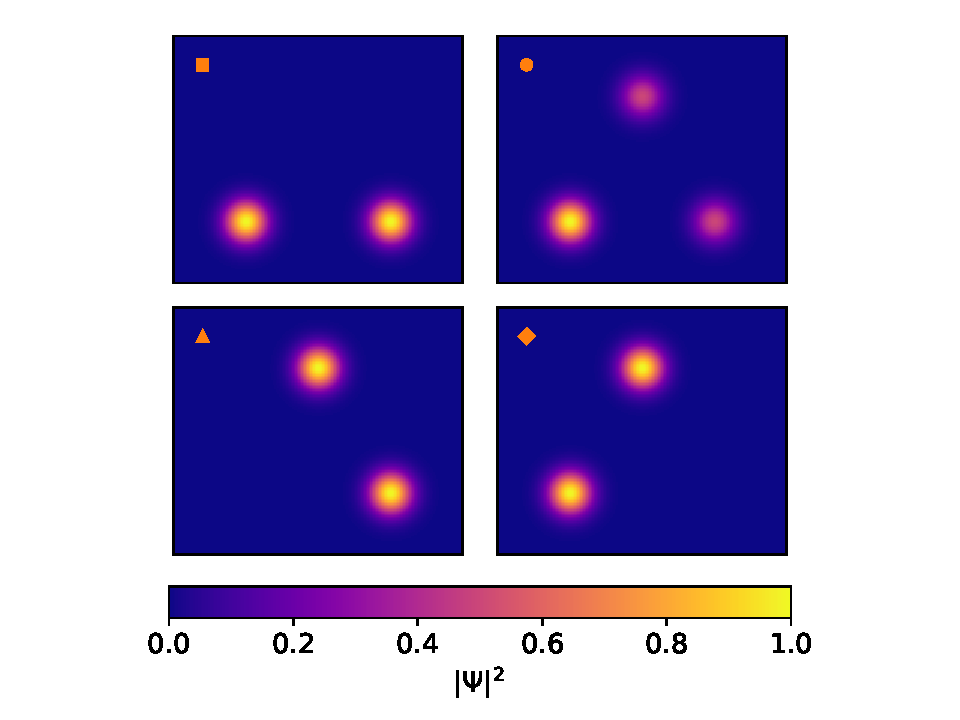
\includegraphics[width=0.6\textwidth]{./figures/3eigvec.pdf}};
    \end{tikzpicture}

  \end{frame}

  \begin{frame}
    \frametitle{Triangular ribbon and topological phases}
    % show spectral plot and wavefunction

    \begin{columns}
      \column{0.5\textwidth}
      \footnotesize
      \begin{equation*}
        \phi_{jl} = \dfrac{e}{\hbar}\int_{\vec{r}_j}^{\vec{r}_l} \vec{A} \cdot d\vec{l} = \vec{A}\cdot\vec{r}_{jl} = -\phi_{lj}
      \end{equation*}
      \vspace{-5mm}
      \begin{figure}
        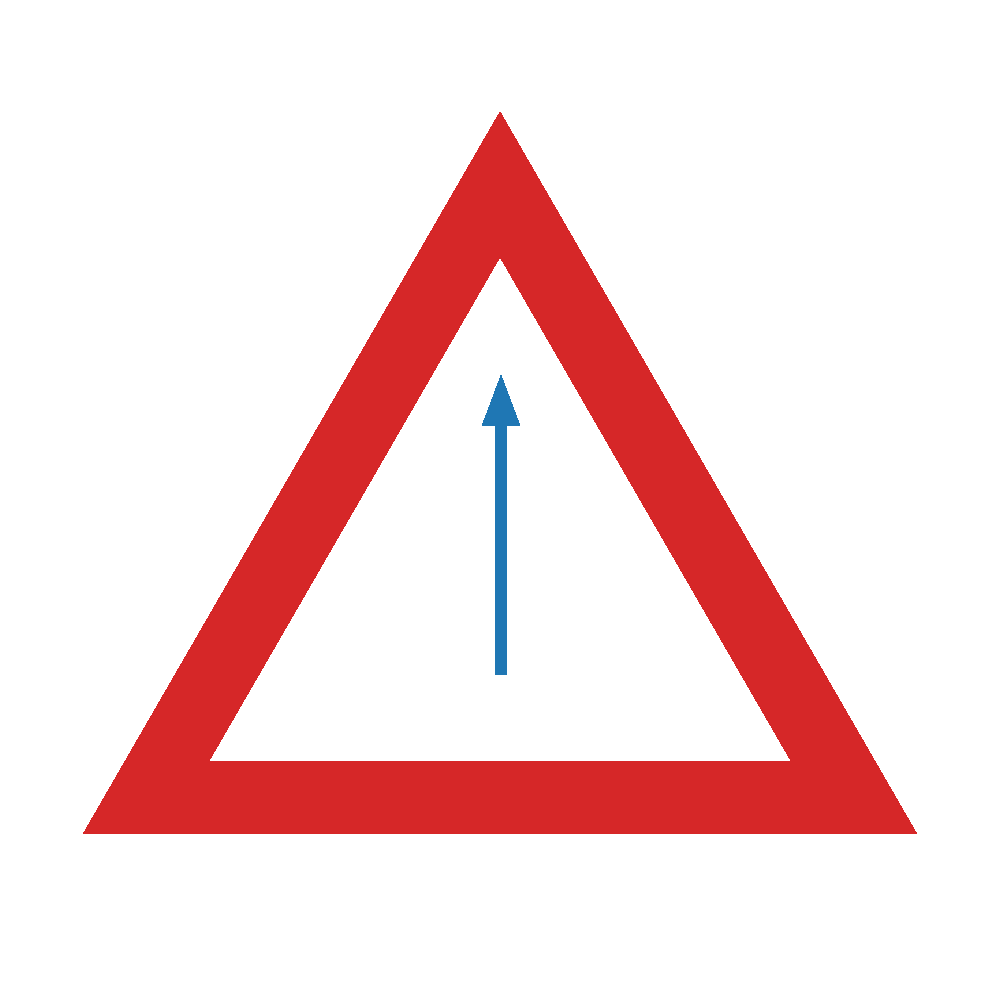
\includegraphics[height=0.50\textheight]{./figures/hollow-triangle-constant-vector-potential.pdf}
      \end{figure}

      \vspace{-10mm}
      \begin{figure}
        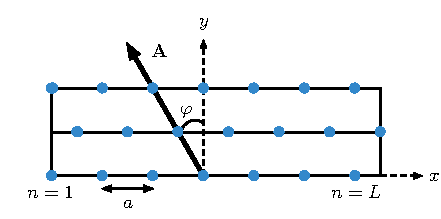
\includegraphics[height=0.30\textheight]{./figures/triangular-lattice-finite-width-ribbon.pdf}
      \end{figure}

      \column{0.5\textwidth}
      \pause

      \begin{figure}
        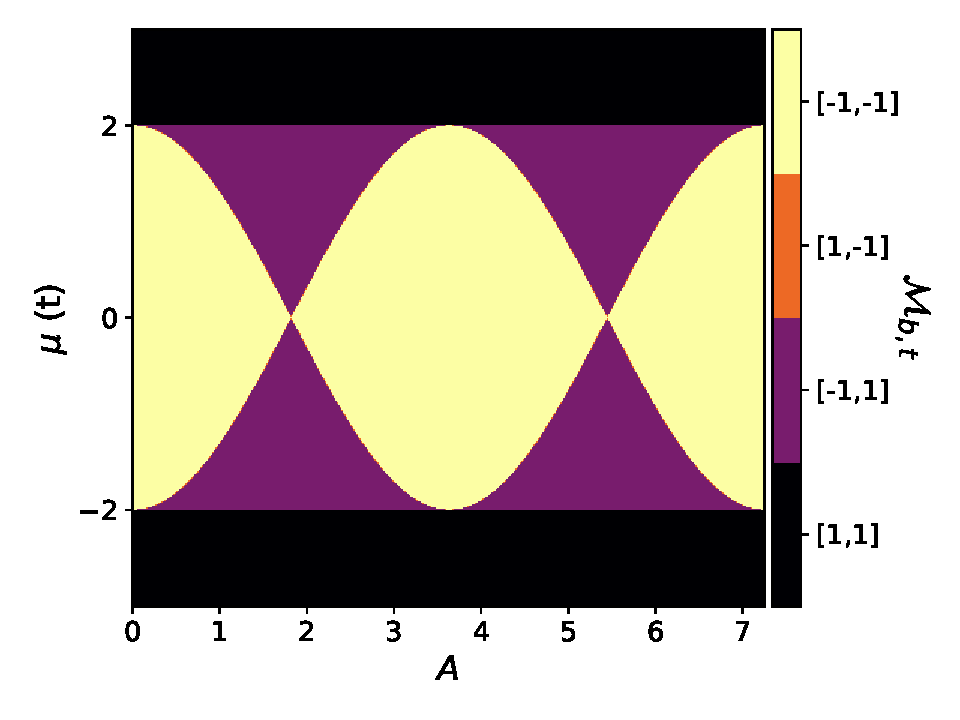
\includegraphics[height=0.45\textheight]{./figures/topological-phase-diagram-1pi3-w-1.pdf} \\
        \hspace{-10mm}
        \pause
        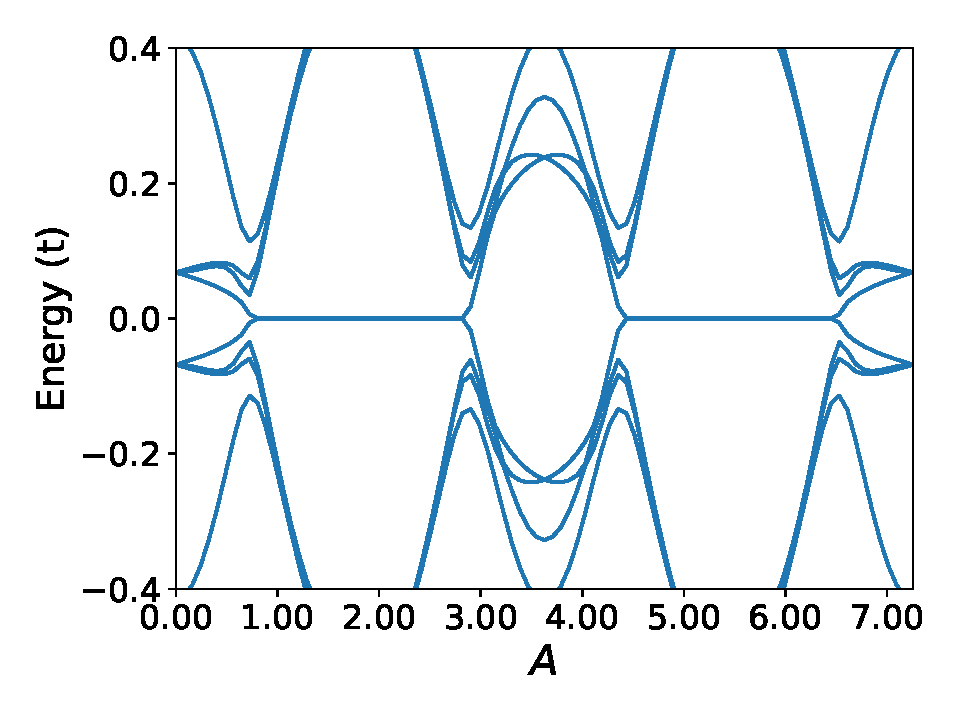
\includegraphics[height=0.39\textheight]{./figures/spectral-flow-nr-50-w-1-mu-1_6.pdf}
      \end{figure}
    \end{columns}

  \end{frame}

  \begin{frame}
    \frametitle{Braiding Majorana zero modes triangular chain (W=1)}

    \begin{figure}
      \begin{tikzpicture}
        \node[inner sep=0pt] (figure) at (-2.8,0){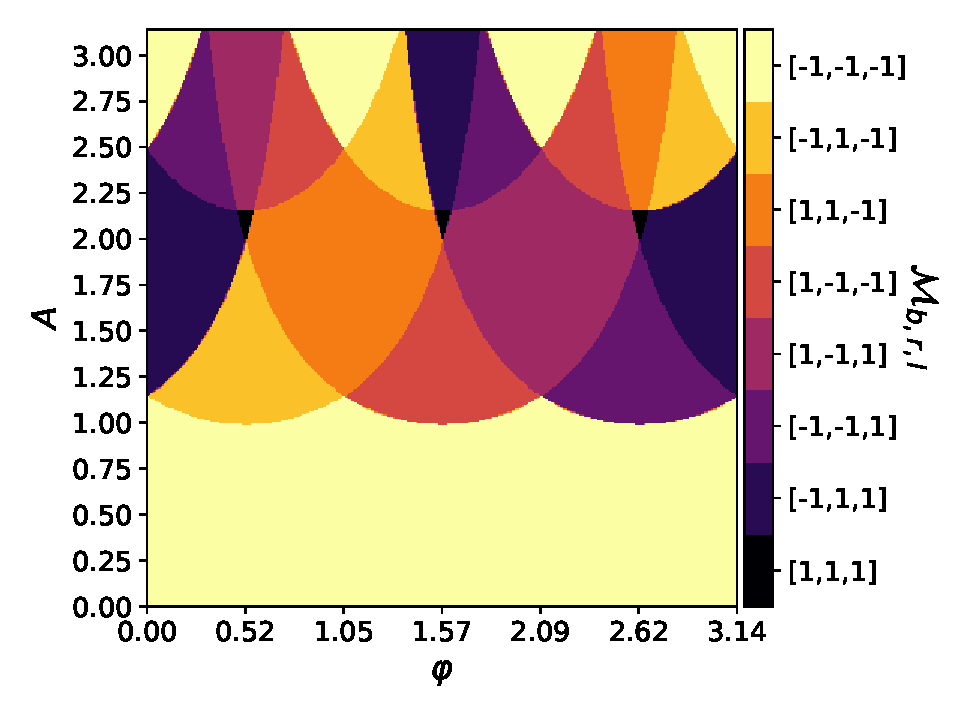
\includegraphics[width=0.4\textwidth]{./figures/topological-phase-diagram-w-1-mu-p1_1000.pdf}};
        \pause
        \draw[line width=0.3mm, green] (-4.75,1.1) -- (-1.3,1.1);
        \pause
        \node[inner sep=0pt] (figure2) at (2.8,0){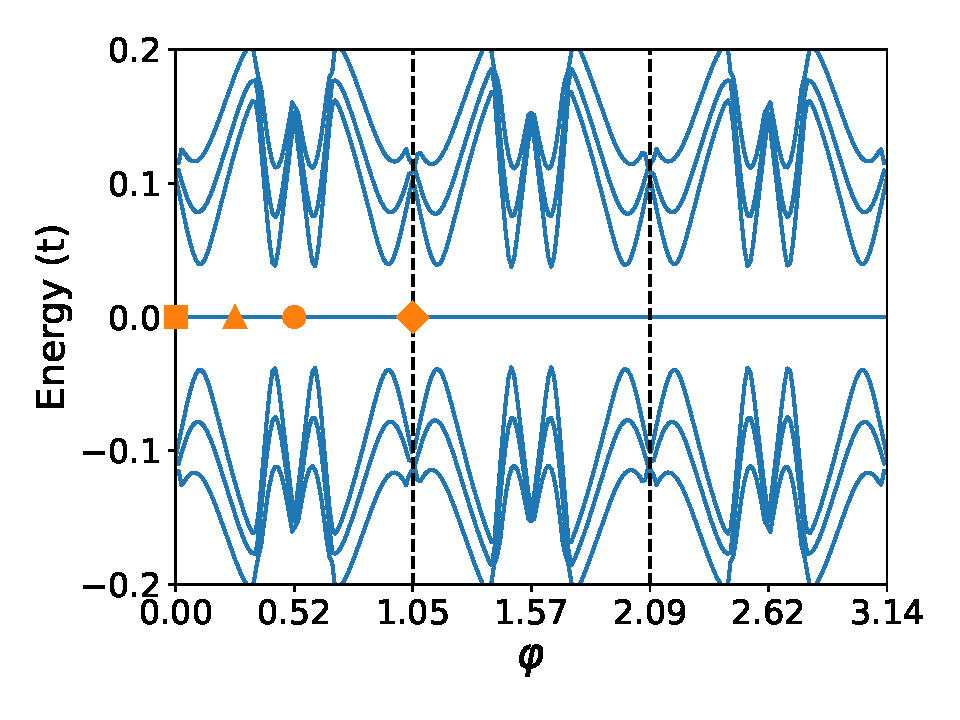
\includegraphics[width=0.4\textwidth]{./figures/spectral-flow-rotation-constant-vector-nr-50-w-1-mu-1_1.pdf}};
        \node[inner sep=0pt] (caption) at (0,-2.0) {\footnotesize $L=50$, $W=1$, $\mu=1.1$, $A=2.35$};
        \onslide<1->
      \end{tikzpicture}
    \end{figure}
    \pause
    \vspace{-2mm}
    \begin{figure}
      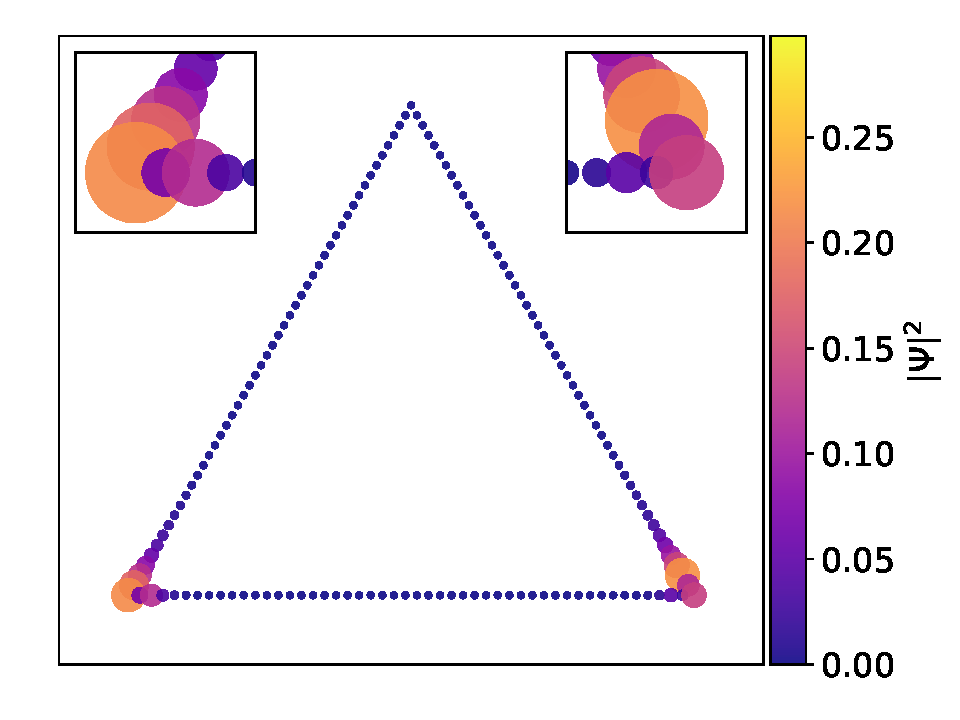
\includegraphics[height=80pt]{./figures/GS-T-Square.pdf}\hspace{-25pt}
      \pause
      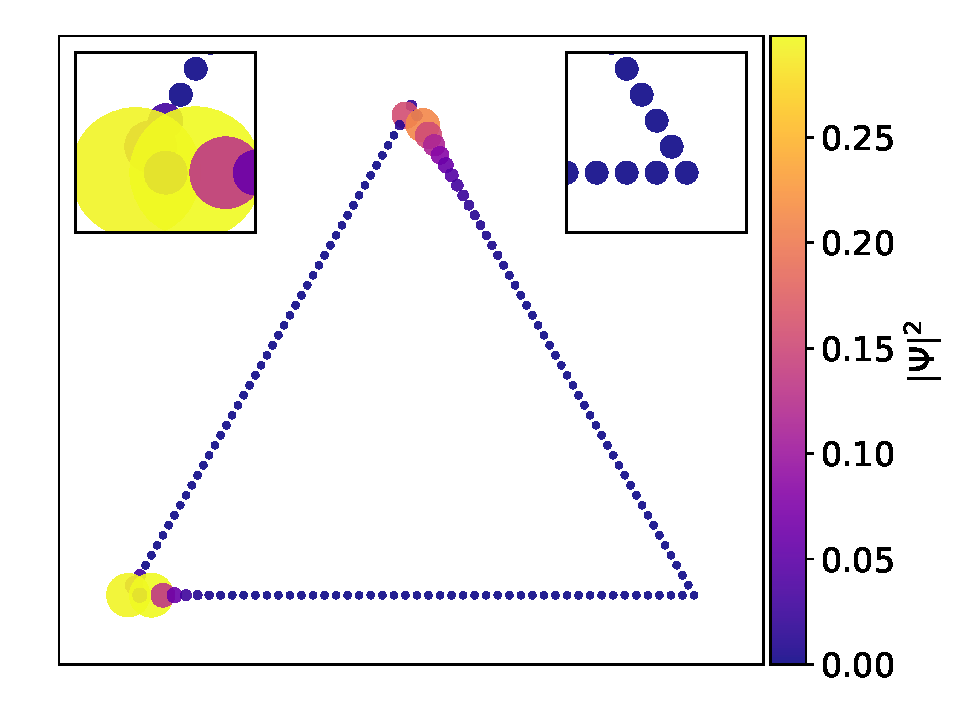
\includegraphics[height=80pt]{./figures/GS-T-Triangle.pdf}\hspace{-25pt}
      \pause
      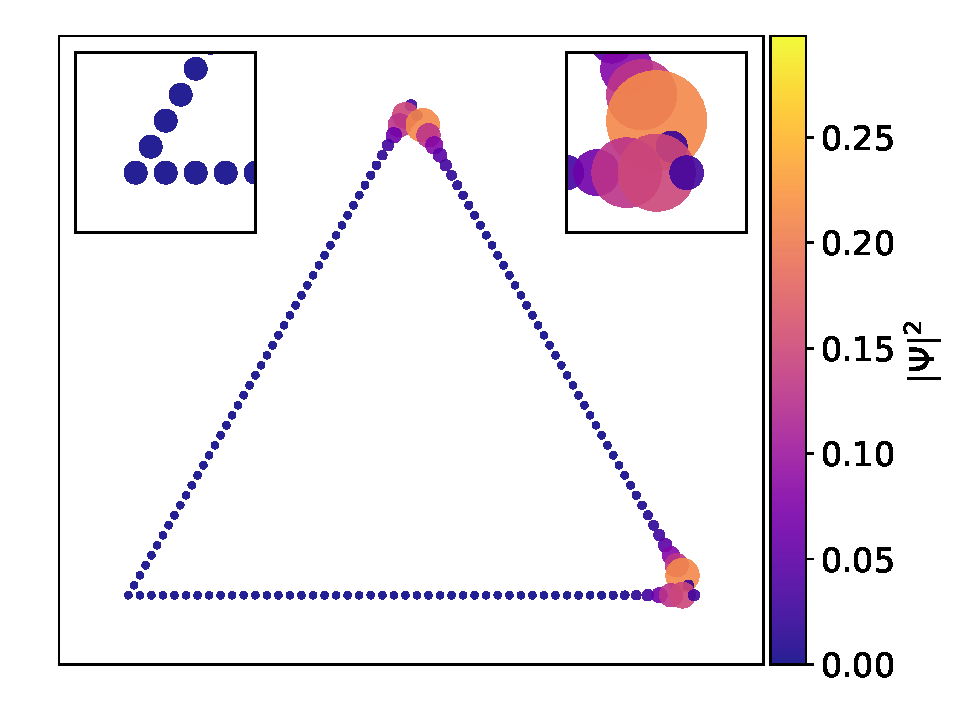
\includegraphics[height=80pt]{./figures/GS-T-Circle.pdf}\hspace{-25pt}
      \pause
      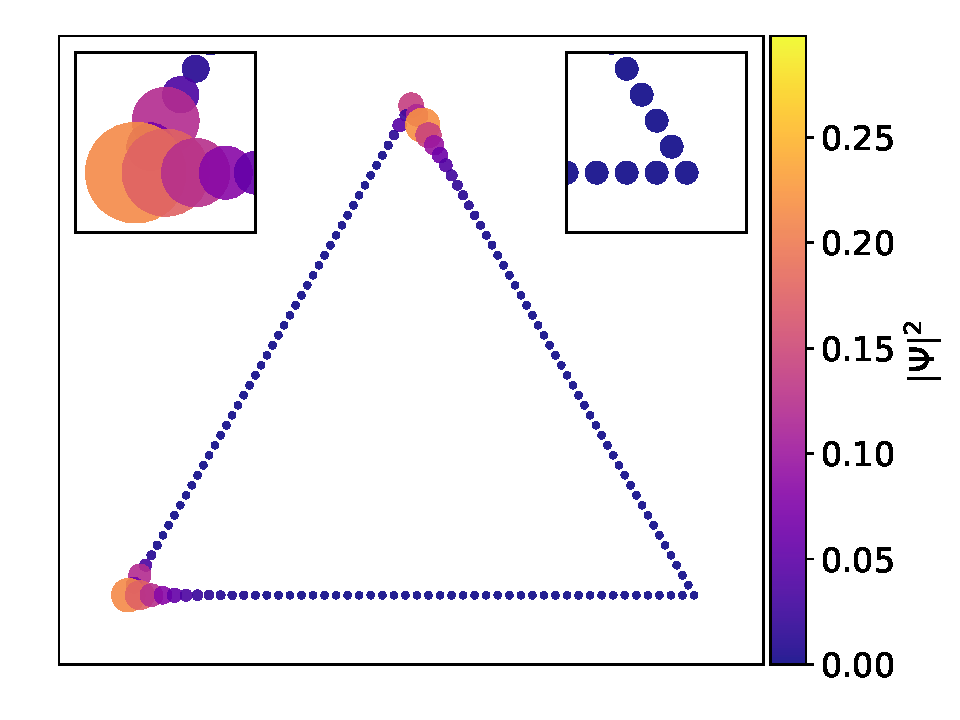
\includegraphics[height=80pt]{./figures/GS-T-Diamond.pdf}
    \end{figure}
  \end{frame}

  \begin{frame}
    \frametitle{Braiding Majorana zero modes hollow triangle (W=3)}

    \begin{figure}
      \begin{tikzpicture}
        \node[inner sep=0pt] (figure) at (-4.5,0.0){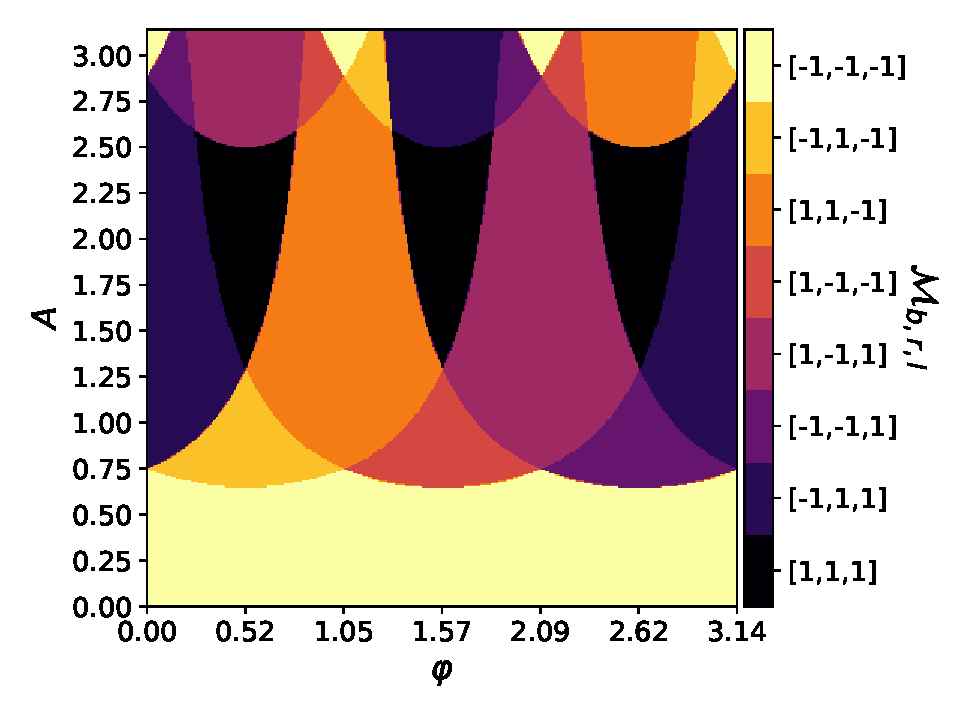
\includegraphics[width=0.33\textwidth]{./figures/topological-phase-diagram-w-3-mu-p1_6000.pdf}};
        \node[inner sep=0pt] (figure2) at (0,0){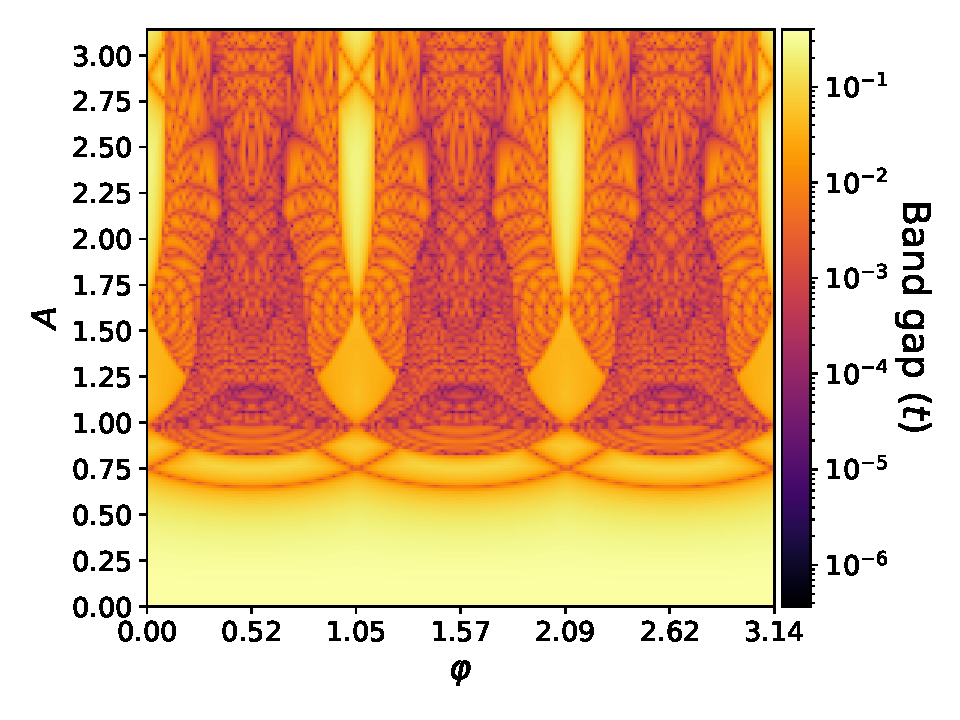
\includegraphics[width=0.33\textwidth]{./figures/band-gap-rotation-w-3-mu-p1_6000.pdf}};

        \visible<2->{
        \draw[line width = 0.2mm, green] (-6.10,-0.43) -- (-5.63,-0.55);
        \draw[line width = 0.2mm, green] (-5.63,-0.55) -- (-5.16,-0.43);

        \draw[line width = 0.2mm, green] (-5.16,-0.43) -- (-4.69,-0.55);
        \draw[line width = 0.2mm, green] (-4.69,-0.55) -- (-4.22,-0.43);

        \draw[line width = 0.2mm, green] (-4.22,-0.43) -- (-3.75,-0.55);
        \draw[line width = 0.2mm, green] (-3.75,-0.55) -- (-3.28,-0.43);

        \draw[line width = 0.2mm, green] (-1.60,-0.43) -- (-1.10,-0.55);
        \draw[line width = 0.2mm, green] (-1.10,-0.55) -- (-0.59,-0.43);

        \draw[line width = 0.2mm, green] (-0.59,-0.43) -- (-0.09,-0.55);
        \draw[line width = 0.2mm, green] (-0.09,-0.55) -- (0.41,-0.43);

        \draw[line width = 0.2mm, green] (0.41,-0.43) -- (0.92,-0.55);
        \draw[line width = 0.2mm, green] (0.92,-0.55) -- (1.42,-0.43);
        }

        \visible<3->{
        \node[inner sep=0pt] (figure3) at (4.5,0){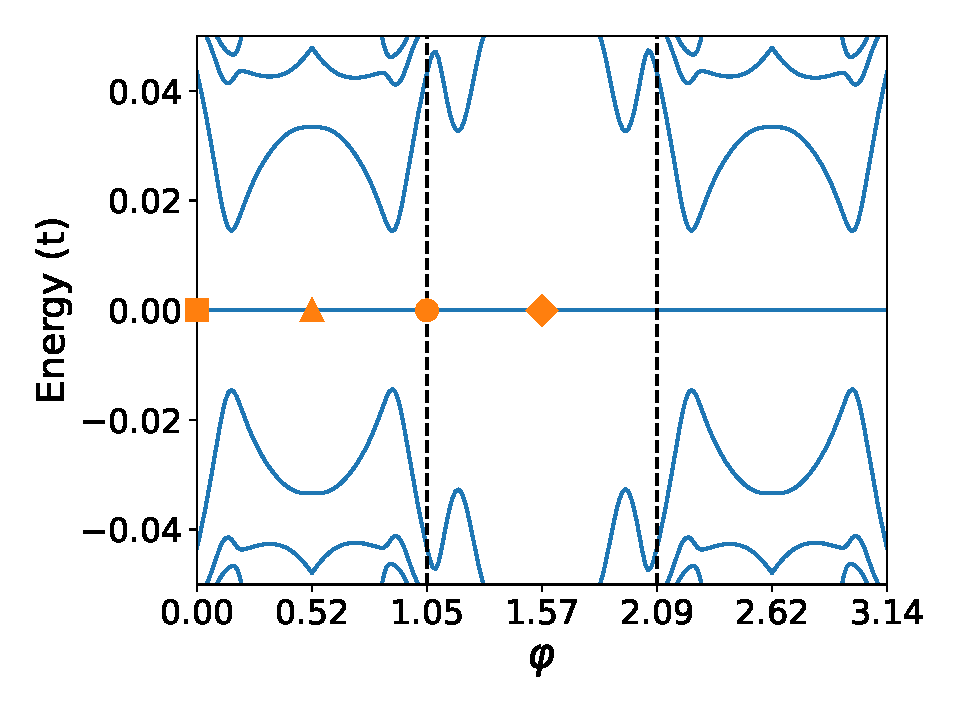
\includegraphics[width=0.33\textwidth]{./figures/spectral-flow-rotation-nr-80-w-3-mu-p1_6000.pdf}};
        \node[inner sep=0pt] (caption) at (0,-2.0) {\footnotesize $L=80$, $W=3$, $\mu=1.6$, $(A,\varphi) = (0.83,0) \rightarrow (0.77,\tfrac{\pi}{6}) \rightarrow (0.83,\tfrac{\pi}{3}) \rightarrow (0.77, \tfrac{\pi}{2}) \dots$};
        }
      \end{tikzpicture}
    \end{figure}

    \visible<4>{
    \begin{figure}
      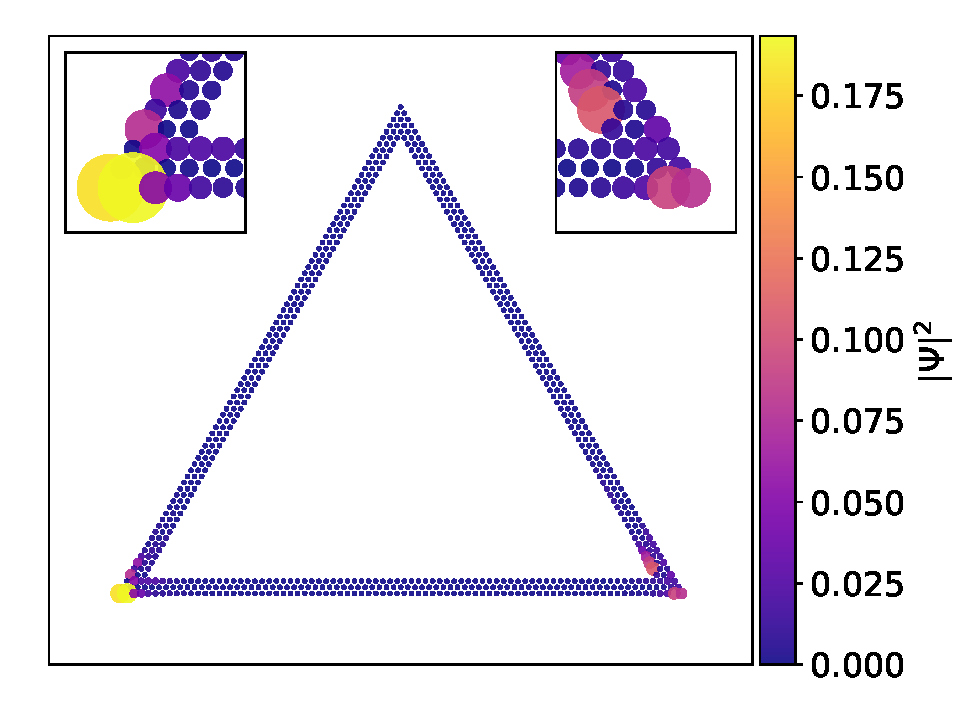
\includegraphics[height=80pt]{./figures/GS-T-Square-w-3.pdf}\hspace{-26pt}
      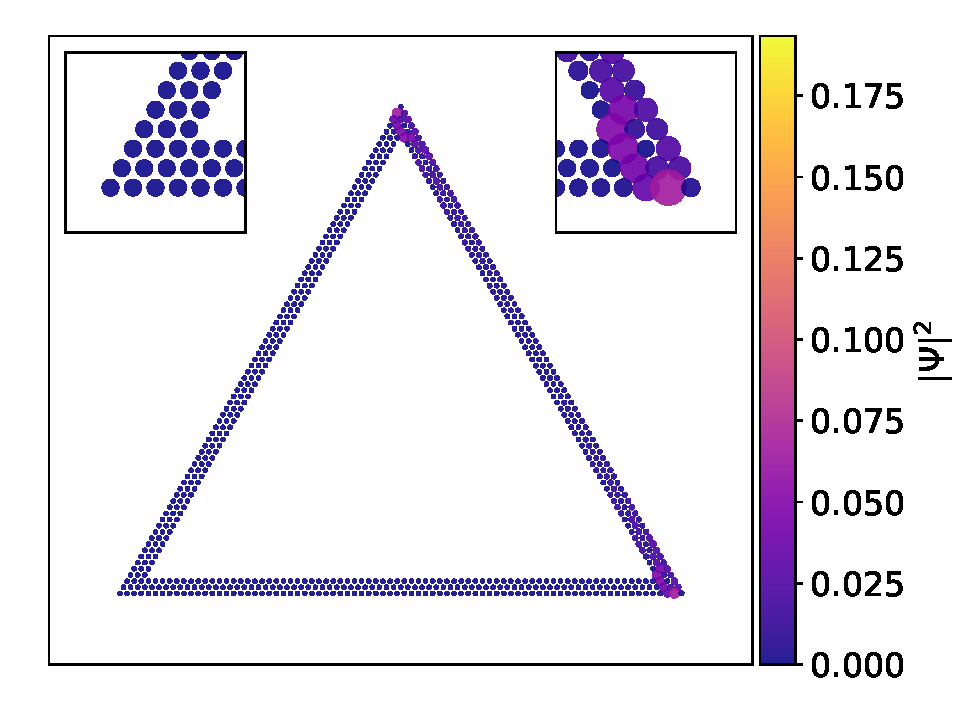
\includegraphics[height=80pt]{./figures/GS-T-Triangle-w-3.pdf}\hspace{-26pt}
      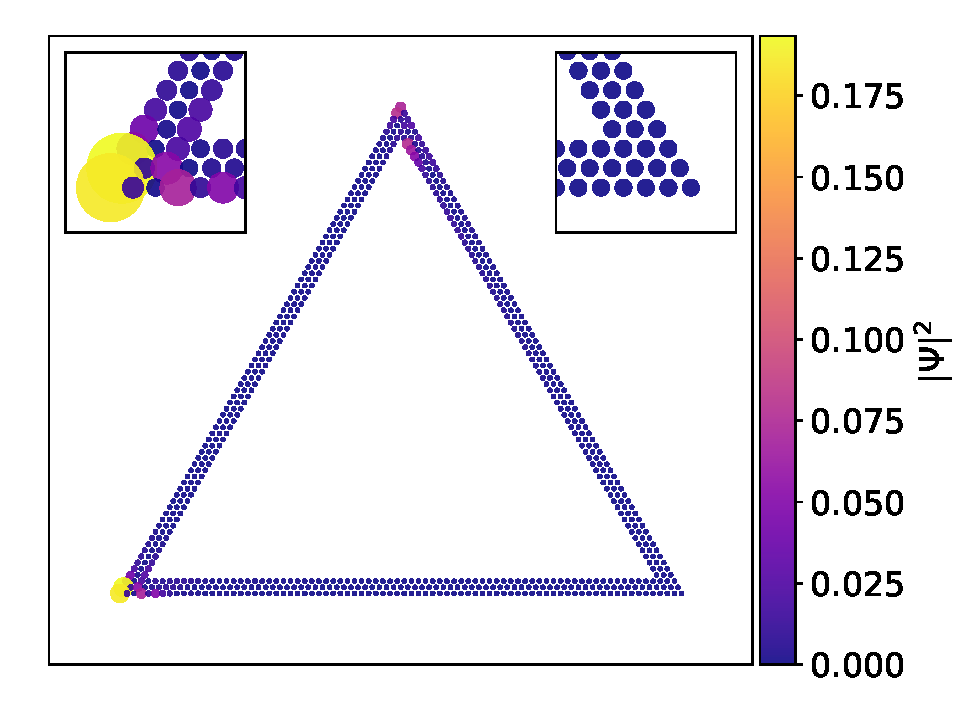
\includegraphics[height=80pt]{./figures/GS-T-Circle-w-3.pdf}\hspace{-26pt}
      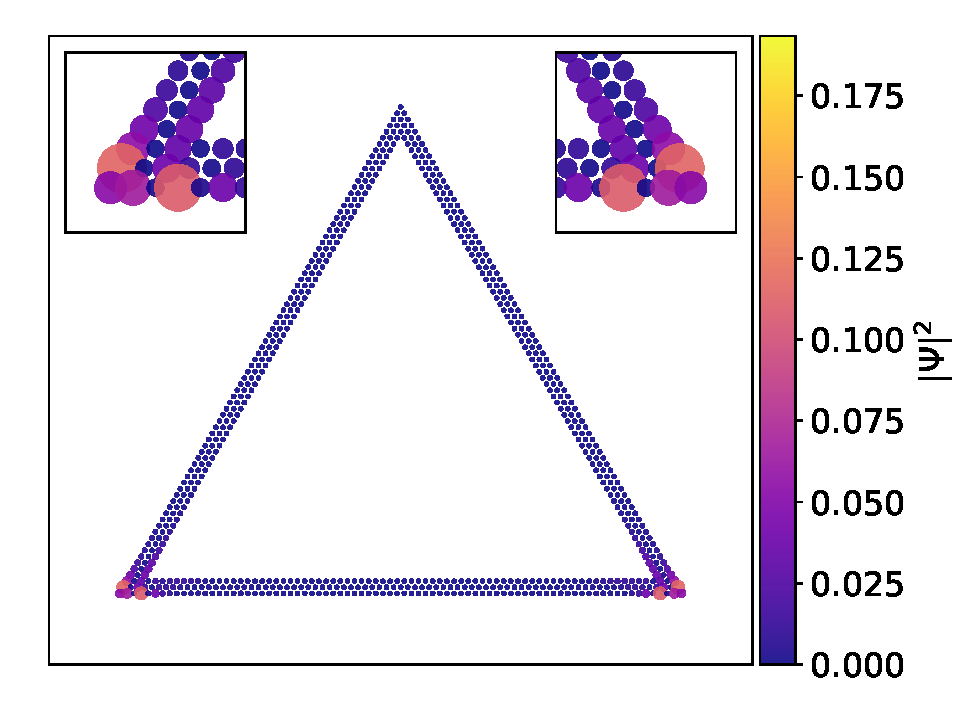
\includegraphics[height=80pt]{./figures/GS-T-Diamond-w-3.pdf}
    \end{figure}
    }

  \end{frame}

  \begin{frame}
    \frametitle{Braiding Two of Four Majorana zero modes}
    \vspace{-2mm}
    \begin{figure}
      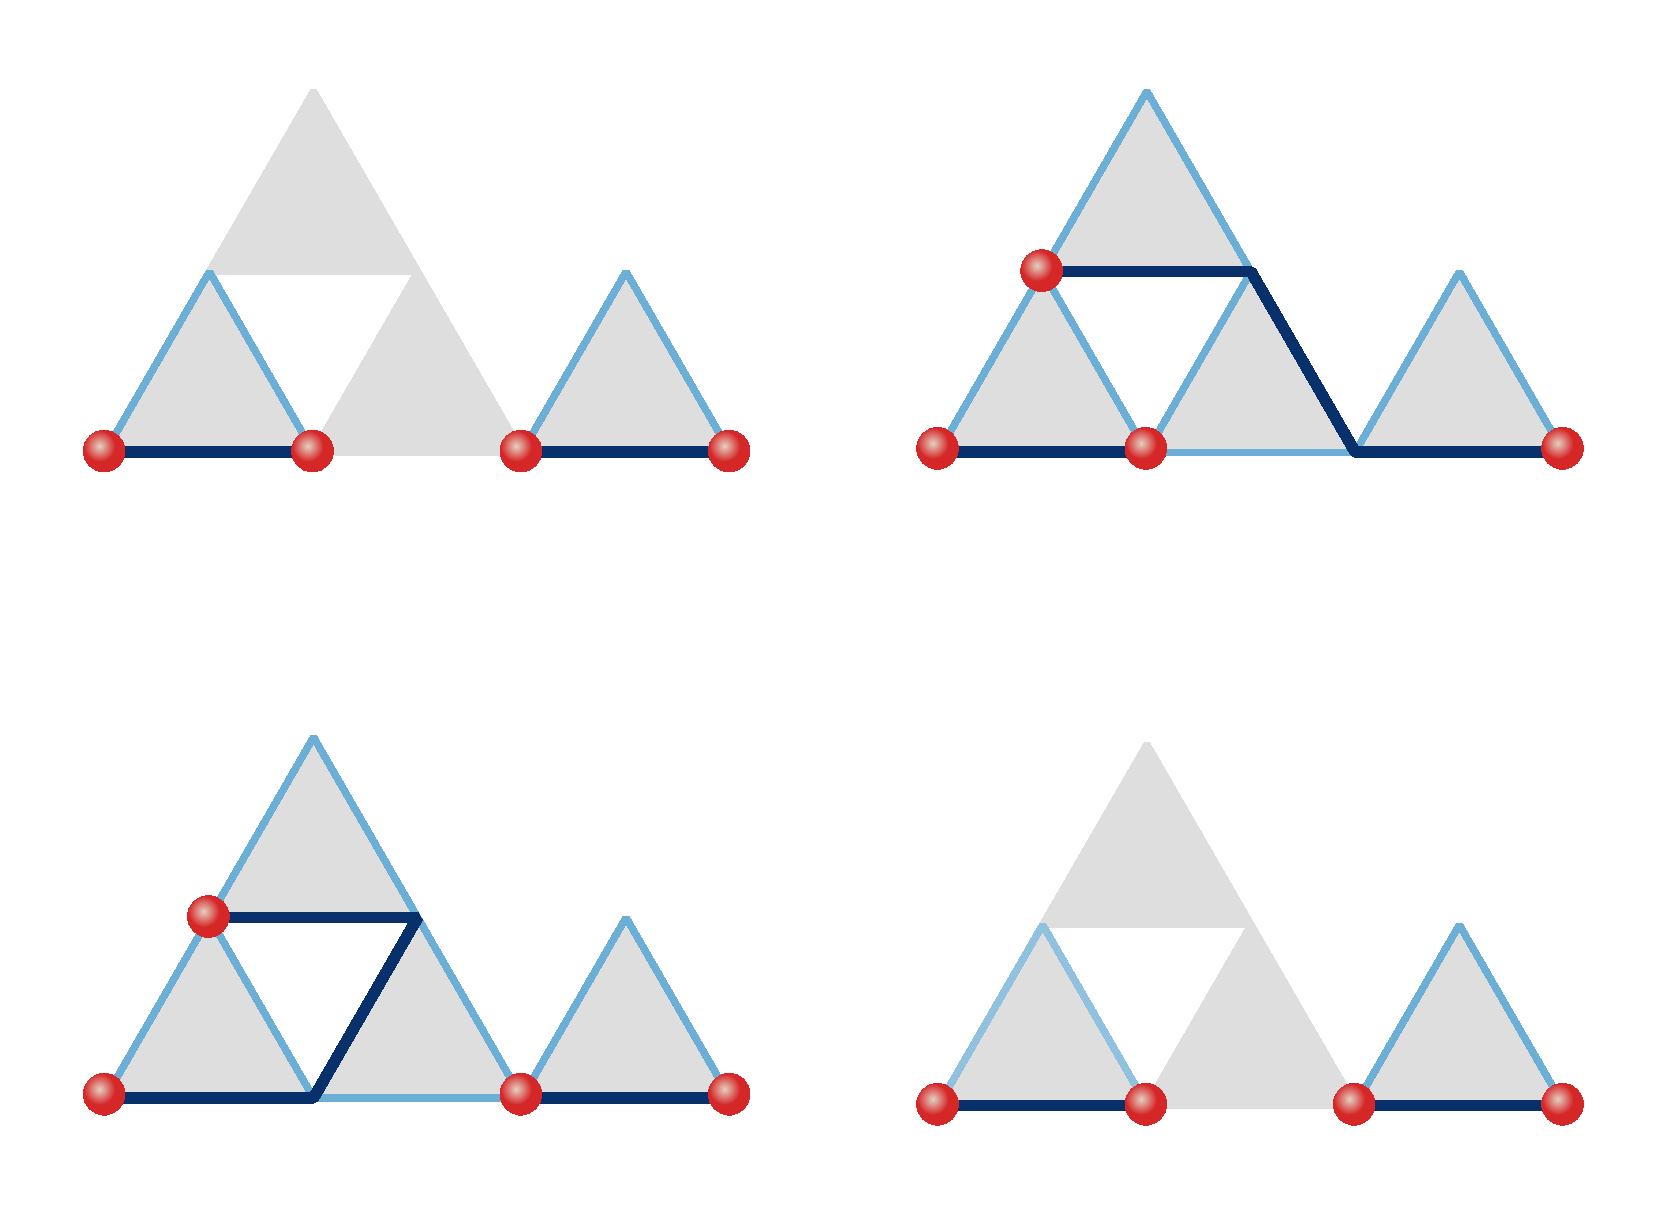
\includegraphics[height=0.9\textheight]{./figures/4-mf-swap-2-3.pdf}
    \end{figure}
  \end{frame}

  %\section{\CO}
  \begin{frame}
    \frametitle{Part I: Summary}

    \begin{itemize}
      \item A minimal Kitaev triangle can emerge as an effective theory for three fermionic sites and is sufficient for braiding.
      \item Hollow triangles maintain 1D bulk-edge correspondence, gauge potential strength and rotation allows for additional topological tunability, and demonstrates braiding.
      \item MZMs can be hosted and braided on a network of triangular islands.
    \end{itemize}
    \vspace{2em}
    \centering
    \small
    Aidan Winblad and Hua Chen, \textit{PRB} \textbf{109}, 205158 (2024).
  \end{frame}

  \section{II: \BD }

  \begin{frame}{Part II: Floquet quantum Hall effect outline}
    \begin{itemize}
      \item Background \& Motivation:
      \begin{itemize}
        \item Quantum Hall effect
        \item Floquet engineering and nonequilibrium physics
      \end{itemize}
      \item Formulation:
      \begin{itemize}
        \item Floquet theorem and high-frequency approximation
        \item Inhomogeneous, circularly polarized light
      \end{itemize}
      \item Results:
      \begin{itemize}
        \item Dirac and 2DEG systems
      \end{itemize}
      \item Summary
    \end{itemize}
  \end{frame}

  \begin{frame}{Quantum Hall effect at the Hall effect Zoo}
    \begin{columns}
      \column{0.5\textwidth}
      \centering
      \begin{tikzpicture}
        \visible<1>{
          \node[inner sep=0pt] (fig) at (0,0) {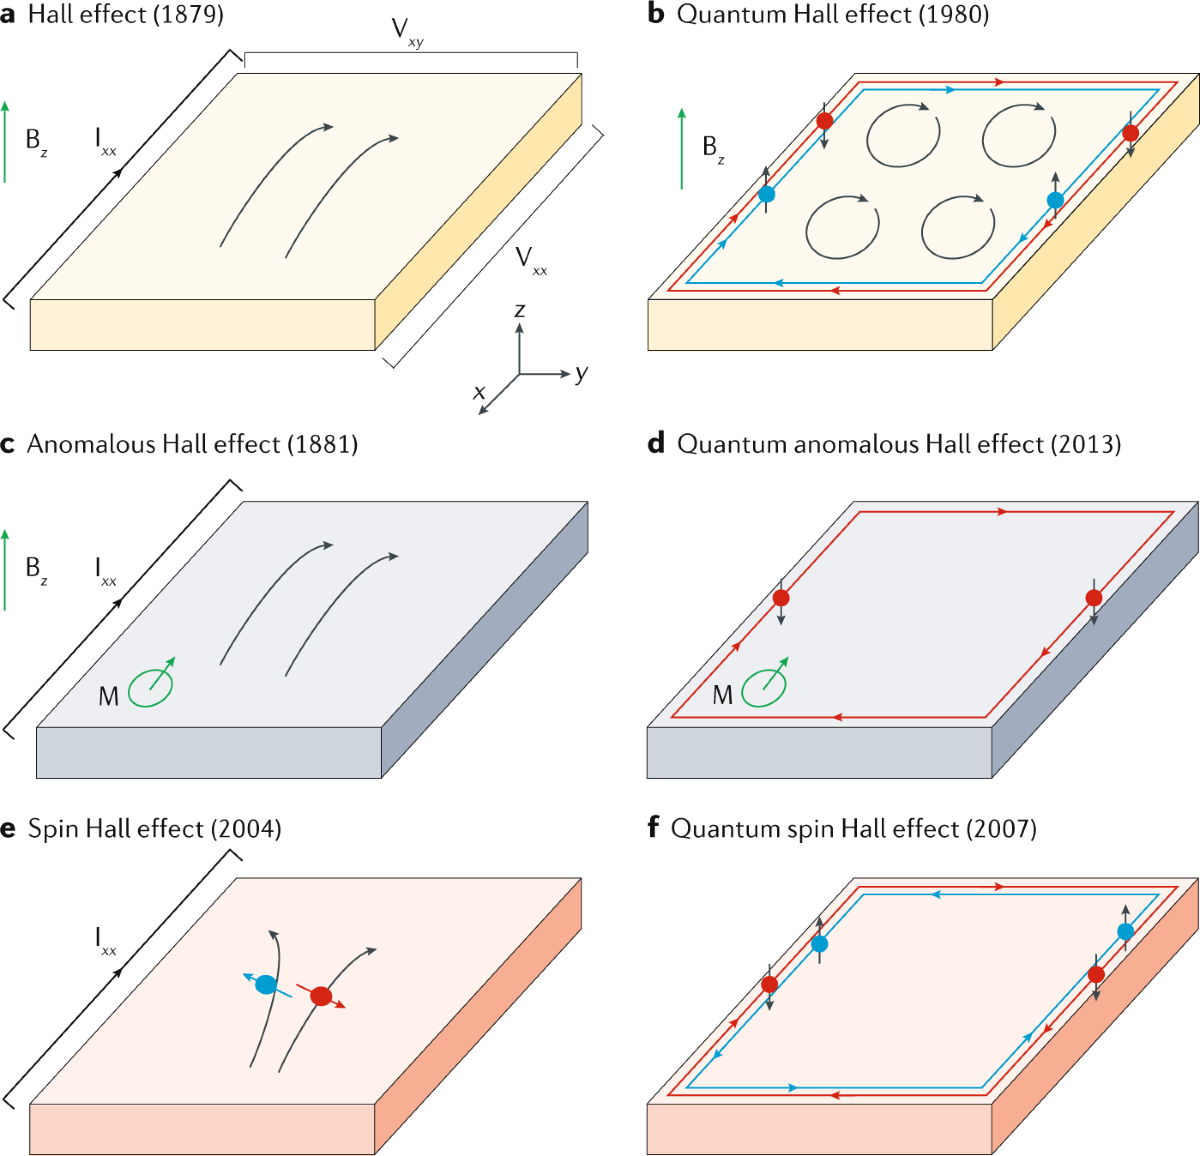
\includegraphics[height=0.75\textheight]{./figures/hall-effects.png}};
          \node[inner sep=0pt] (ref) at (0,-3.45) {\footnotesize von Klitzing et al.\, \textit{Nat.\ Rev.\ Phys.} \textbf{2}, 397-401 (2020)};
        }
        \visible<2->{
          \node[inner sep=0pt] (fig) at (0,2) {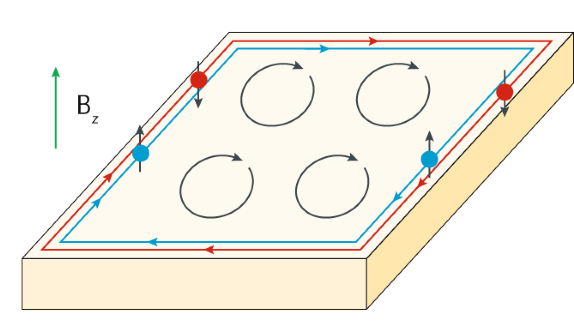
\includegraphics[height=0.4\textheight]{./figures/quantum-hall-effect.png}};
        }
        \visible<3->{
          \node[inner sep=0pt] (fig) at (0,-1.5) {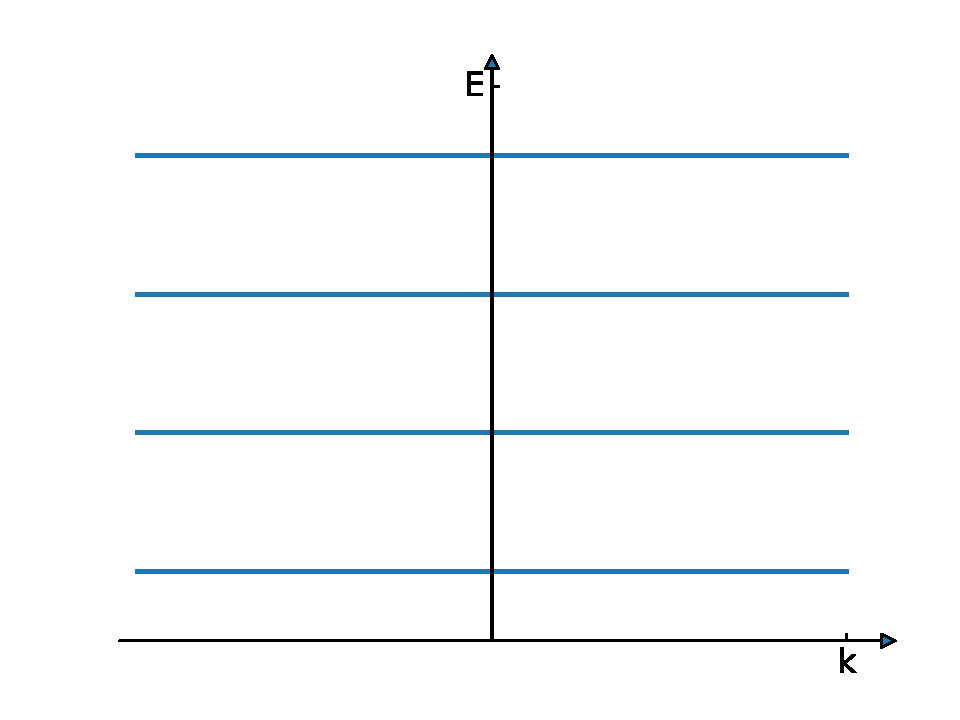
\includegraphics[height=0.45\textheight]{./figures/qhe-unfilled-bands.pdf}};
        }
        \visible<4->{
          \node[inner sep=0pt] (fig) at (0,-1.5) {\includegraphics[height=0.45\textheight]{./figures/qhe-filled-bands.pdf}};
        }
      \end{tikzpicture}

      \column{0.5\textwidth}
      \visible<2->{
        \small
        \centering
        %Dirac Hamiltonian with uniform magnetic field
        \begin{equation*}
          \text{Dirac: }
          \begin{cases}
            \ham^{D} = v_F \bm{\sigma}\cdot \left(\vec{p} + eBx\hat{y}\right) \\ \\
            \epsilon_n^{D} = \pm v_F \sqrt{ 2 n \hbar e B }
          \end{cases}
        \end{equation*}
        \newline
      }
      \visible<2->{
        %2DEG Hamiltonian with uniform magnetic field
        \begin{equation*}
          \text{2DEG: }
          \begin{cases}
            \ham^{\text{2DEG}} = \dfrac{1}{2m^*} {\left(\vec{p} + eBx\hat{y}\right)}^2 \\ \\
            \epsilon_n^{\text{2DEG}} = \dfrac{\hbar e B}{m^*} \left( n + \dfrac{1}{2} \right)
          \end{cases}
        \end{equation*}
      }
      \visible<4->{
        \centering
        \newline
        \textbf{QHE has quantized Hall conductance:} \newline $\sigma_H = -\dfrac{Ce^2}{h}$
      }
    \end{columns}
  \end{frame}

  \begin{frame}{Floquet exhibit at the Hall effect Zoo}
    \textbf{Pioneer research on nonequilibrium systems exhibiting equilibrium physics.}
    \newline
    \textbf{Circularly polarized light provides time periodicity to use Floquet theorem and high-frequency approximation.}
    \newline
    \begin{itemize}
      \item Photovoltaic Hall effect in graphene
      \begin{itemize}
        \item \small Oka et al., \textit{PRB} \textbf{79}, 0814406(R) (2009)
      \end{itemize}
      \item Floquet topological insulator in semiconductor quantum wells
      \begin{itemize}
        \item \small Lindner et al., \textit{Nat. Phys.} \textbf{7}, 490-495 (2011)
      \end{itemize}
      \item Observations of Floquet-Bloch states on the surface of a topological insulator
      \begin{itemize}
        \item \small Wang et al., \textit{Science} \textbf{342}, 453-457 (2013)
      \end{itemize}
      \item Floquet Fractional Chern Insulators
      \begin{itemize}
        \item \small Grushin et al., \textit{PRL} \textbf{112}, 156801 (2014)
      \end{itemize}
    \end{itemize}

  \end{frame}

  \begin{frame}{Floquet quantum anomalous Hall effect}
    \begin{columns}
      \column{0.5\textwidth}
      \centering
      \begin{figure}
        \includegraphics[width=0.95\textwidth]{./figures/kitagawa-theory.png}
        %\caption*{\footnotesize Transport properties of nonequilibrium systems under the application of light: photoinduced quantum Hall insulators without Landau levels. Kitagawa et.\ al., \textit{PRB} \textbf{84}, 235108 (2011)}
        %\caption*{\footnotesize Photoinduced quantum Hall insulators without Landau levels. Kitagawa et.\ al., \textit{PRB} \textbf{84}, 235108 (2011)}
        \caption*{\footnotesize Kitagawa et.\ al., \textit{PRB} \textbf{84}, 235108 (2011)}
      \end{figure}

      \column{0.5\textwidth}
      \visible<2>{
      \begin{figure}
        \includegraphics[width=0.85\textwidth]{./figures/fqahe-dirac.png}
        %\caption*{\footnotesize Light-induced anomalous Hall effect in graphene. McIver et.\ al., \textit{Nature Phys.} \textbf{16}, 38 (2020)}
        \caption*{\footnotesize McIver et.\ al., \textit{Nature Phys.} \textbf{16}, 38 (2020)}
      \end{figure}
      }
    \end{columns}
  \end{frame}

  \section{II:\ \FO}

  \begin{frame}{Floquet Theorem}
    \centering
    \textbf{Analogous to Bloch's theorem}
    \vspace{1em}
    \begin{columns}
      \column{0.5\textwidth}
      \small
      \centering
      \visible<2->{
        Exhibits discrete time translation symmetry
        \begin{equation*}
          H(t+T) = H(t)
        \end{equation*}
      }
      \visible<3->{
        For such a system, Floquet theorem must hold
        \begin{gather*}
          \psi_{\epsilon}(t) = e^{-i\epsilon t / \hbar} u_{\epsilon}(t) \\
          u_{\epsilon}(t+T) = u_{\epsilon}(t)
        \end{gather*}
        Let wavefunction be an arbitrary wave approximation
        \begin{gather*}
          \psi(t) = \sum_{\epsilon} u_{\epsilon} e^{-i\epsilon t / \hbar}
        \end{gather*}
      }
      \column{0.5\textwidth}
      \small
      \centering
      \visible<4->{
        Discrete time Fourier series of Hamiltonian
        \begin{gather*}
          H(t) = \sum_{n} H_n e^{in\omega t}
        \end{gather*}

        Where
        \begin{gather*}
          H_n = \frac{1}{T} \int_0^T H(t) e^{-in\omega t}
        \end{gather*}
      }
      \visible<5->{
        Then, $i\hbar \partial_t \psi(t) = H(t) \psi(t)$ becomes
        \begin{gather*}
          \bar Q_{m,m+n} = H_n - m\hbar\omega\delta_{n0}
        \end{gather*}
      }
    %\vspace{5mm}
    \end{columns}
    \centering
    \visible<6>{
      \textbf{$\bar Q$ is an infinite quasienergy matrix! How do we handle such a matrix?}
    }
  \end{frame}

  \begin{frame}{Quasienergy operator and high-frequency approximation}
    \begin{columns}
      \small
      \column{0.45\textwidth}
      \visible<1->{
        \[
        \bar Q =
        \begin{bmatrix}
          \ddots & \vdots & \vdots & \vdots & \reflectbox{$\ddots$} \\
          \cdots &  H_0 - \hbar \omega  &  H_{-1} &  H_{-2} & \cdots \\
          \cdots &  H_{1}  &  H_0 &  H_{-1} & \cdots \\
          \cdots &  H_{2}  &  H_1 &  H_{0} + \hbar \omega & \cdots \\
          \reflectbox{$\ddots$} & \vdots & \vdots & \vdots & \ddots \\
        \end{bmatrix}
        \]
      }

      \column{0.2\textwidth}
      \centering
      \visible<2->{
        $\rightarrow$ \fcolorbox{red}{white}{$H_{\pm n} \ll \hbar \omega$} $\rightarrow$
      }

      \column{0.45\textwidth}
      \visible<3->{
        \begin{bmatrix}
          \ddots & \vdots & \vdots & \vdots & \reflectbox{$\ddots$} \\
          \cdots &  H_{\text{eff}} - \hbar \omega  & 0 & 0 & \cdots \\
          \cdots & 0  &  H_{\text{eff}} & 0 & \cdots \\
          \cdots & 0  & 0 &  H_{\text{eff}} + \hbar \omega & \cdots \\
          \reflectbox{$\ddots$} & \vdots & \vdots & \vdots & \ddots \\
        \end{bmatrix}
      }
    \end{columns}
    \small
    \centering
    \visible<4->{
      \begin{gather*}
        H_{\text{eff}} = H^{F(1)} + H^{F(2)} + H^{F(3)} + \dots
      \end{gather*}
      \begin{align*}
        H^{F(1)} &= H_0 \\
        H^{F(2)} &= \sum_{m> 0} \frac{2[H_m, H_{-m}]}{m\hbar\omega} \\
        H^{F(3)} &= \sum_{m> 0} \left( \frac{[H_{-m} , [H_0, H_m]] + h.c.}{2(m\hbar\omega)^2} + \sum_{m'\neq m} \frac{[H_{-m'}, [H_{m'-m}, H_m]] + h.c.}{3mm'(\hbar\omega)^2} \right)
      \end{align*}
    }
  \end{frame}

  \begin{frame}{Inhomogeneous, circularly polarized light on 2D systems}
    \begin{figure}
      \includegraphics[height=0.4\textheight]{./figures/fll-setup.pdf}
    \end{figure}
    Generalized electric field at substrate surface
    \begin{align*}
      \small
      %\vec{E}_1 &= E\cos{(a\omega t)} \hat{x},\\
      %\vec{E}_2 &= \vec{E}_2^f + \vec{E}_2^b = -E\cos{(Kx)}\sin{(b\omega t)} \hat{y}
      %\vec{E}_2 &= -E\cos{(Kx)}\sin{(b\omega t)} \hat{y}
      \vec{E} &= E \langle \cos{(a\omega t)},-\cos{(Kx)}\sin{(b\omega t)} \rangle
    \end{align*}
    where
    \begin{equation*}
      \small
      K = \frac{\omega \sin{(\theta_i)}}{v_p}
    \end{equation*}

  \end{frame}

  \section{II:\ \RE}

  \begin{frame}{Dirac systems}

    \visible<1->{
    \begin{gather*}
      \ham (t) = v_F \bm{\sigma} \cdot \left(\vec{p} + e \vec{A}(t)\right) \\
      \vec{E} = E\langle \cos{(\omega t)}, \sin{(Kx)}\sin{(2\omega t)} \rangle
    \end{gather*}
    }
    \visible<2->{
    \centering
    Use floquet theorem and high-frequency approximation, and in limit $Kx\ll1$
    \begin{gather*}
      \ham_{\text{eff}}^{D} = v_F \sigma_x p_x + v_F \sigma_y \left( C p_y + eB^Dx \right) \\
      B^{D} = \frac{K v_F^2 e^2 E^3}{4\hbar^2 \omega^5}
    \end{gather*}
    }
    %where $C = 1 - {\left(\tfrac{v_F eE}{\hbar \omega^2}\right)}^2$ and
  \end{frame}

  \begin{frame}{2DEG systems}

    \visible<1->{
    \begin{gather*}
      \ham (t) = \dfrac{1}{2m^*} {\left( \vec{p} +e \vec{A}(t)\right)}^2 \\
      \vec{E} = E\langle\cos{(\omega t)}, -\cos{(Kx)}\sin{(\omega t)}\rangle
    \end{gather*}
    }
    \visible<2->{
      \centering
      Use floquet theorem and high-frequency approximation, and in limit $Kx\ll1$
    \begin{gather*}
      \ham_{\text{eff}}^{\text{2DEG}} = \frac{1}{2m^*} \left[ p_x^2 + {\left(p_y - eB^{\text{2DEG}}x \right)}^2\right] \\
      B^{\text{2DEG}} = \frac{K^2 e E^2}{m^* \omega^3}
    \end{gather*}
    }
    \visible<3>{
      \centering
      \textbf{Effective Hamiltonians are approximations, energies and states are Landau level like.}
    }
  \end{frame}

  \begin{frame}{Expected analytical values and tight-binding models}
    \centering
    \begin{itemize}
      \item Parameters from previous literature can produce effective magnetic fields on the order of mT to hundreds of mT in Dirac and 2DEG.
      \item Tight-binding models were performed for both systems
      \begin{itemize}
        \item Strong agreement with high-frequency approximation.
        \item Interpreting data of lower frequencies is difficult and inconclusive when modes overlap.
      \end{itemize}
    \end{itemize}

  \end{frame}

  \begin{frame}{Part II: \CO}
    \begin{itemize}
      \item Inhomogeneous, circularly polarized light induces QHE in Dirac and 2DEG systems.
      \item Showed nonequilibrium systems exhibit equilibrium physics.
      \item Effective magnetic field can be enhanced by several parameters.
    \end{itemize}

  \end{frame}

  \appendix
  \section{Appendix}

  \begin{frame}{Acknowledgments}
    \centering
    \begin{tikzpicture}
      \node[inner sep=0pt] (csu) at (-2,0)
      {\includegraphics[width=2.5cm]{./figures/CSU-Ram-357-617.png}};
      \node[inner sep=0pt] (nsf) at (2,0)
      {\includegraphics[width=2.5cm]{./figures/nsf.png}};
    \end{tikzpicture}
    \vspace{2em}
    \begin{itemize}
      \small
      \item Advisor: Dr. Hua Chen
      \item Committee: Dr. Martin Gelfand, Dr. Richard Eykholt, Dr. Olivier Pinaud
      \item Informative Discussions: Chris Ard and Muhammad Tahir
      \item Friends and Family
      \item CSU Mental Health Services
    \end{itemize}
  \end{frame}

  \begin{frame}
    \frametitle{Additional results from Schneider et al.}

    \begin{figure}
      \includegraphics[height=0.8\textheight]{./figures/Schneider-additional-results.pdf}
    \end{figure}

  \end{frame}

  \begin{frame}
  \frametitle{Majorana fermion notation and coupling isolation}
    The complex fermion operator can be written as a superposition of two Majorana fermions $c_j = \frac{1}{2} (a_j + i b_j)$.
    Due to the nature of Majorana fermions, $a^{\dagger}_j = a_j$, the creation operator is $\cc_j = \frac{1}{2} (a_j - i b_j)$.
    \begin{align*}
      H = -\dfrac{i\mu}{4} \sum_j (a_j b_j - b_j a_j) - \dfrac{i}{4} \sum_{<j,l>} [&(t\sin\phi-\de\sin\theta) a_l a_j + (t\sin\phi+\de\sin\theta) b_l b_j \nonumber \\
      +&(t\cos\phi+\de\cos\theta) a_l b_j - (t\cos\phi-\de\cos\theta) b_l a_j].
    \end{align*}
    \begin{align}
      &(t \sin\phi_{j,l} - \de \sin\theta_{j,l}) a_l a_j, \\
      &(t \sin\phi_{j,l} + \de \sin\theta_{j,l}) b_l b_j, \\
      &(t \cos\phi_{j,l} + \de \cos\theta_{j,l}) a_l b_j, \\
      &(t \cos\phi_{j,l} - \de \cos\theta_{j,l}) b_l a_j
    \end{align}
  \end{frame}

  \begin{frame}
  \frametitle{Gauge potentials in Hamiltonians}

  %\begin{multicols}{2}
  \centering Minimal Coupling
  \begin{gather}
    \vec{p}_{\text{can}} = \vec{p}_{\text{kin}} + q\vec{A} \\
    \ham = \dfrac{1}{2m} {\left( \vec{p}_{\text{can}} - q\vec{A} \right)}^2 + qV
  \end{gather}
  \vspace{1em}

  \centering Peierls Phase
  \begin{gather}
    \cc_j c_l \rightarrow \cc_j c_l \exp{\left[ \dfrac{iq}{\hbar} \int_{\vec{r}_j}^{\vec{r}_j} \vec{A}\cdot d\vec{l} \right]} = e^{i\phi_{jl}} \cc_j c_l \\
    \ham = \sum_{\langle j, l \rangle} t e^{i\phi_{jl}} \cc_j c_l + h.c.
  \end{gather}

  %\end{multicols}

  \end{frame}

  \begin{frame}{Braiding in a 2D \textit{p}-wave superconductor}
    \footnotesize
    \begin{multicols}{2}
      \begin{itemize}
        \item \textit{p}-wave superconductors can exhibit half-quantum vortices.
        \item Triplet pairing
          \begin{equation*}
            \vec{d}(\vec{k}) = \Delta e^{i\phi} \langle \cos \alpha, \sin \alpha, 0 \rangle(k_x + i k_y)
          \end{equation*}
        \item The order phase $\phi$ and angle $\alpha$ of $\vec{d}$ rotate by $\pi: (\phi,\vec{d}) \mapsto (\phi+\pi, -\vec{d})$.
        \item The order parameter $\theta$ maps to itself, $(0,2\pi)$, under the simultaneous change of both \vec{d} and $\phi: \theta = \phi+\alpha$.
      \end{itemize}
      \begin{equation*}
        \ham_{\Delta} = \int d^2\vec{r} \Delta \left[ \Psi^{\dagger} \left[ e^{i\theta} * (\partial_x + i\partial_y) \right] \Psi + h.c. \right]
      \end{equation*}
      %\vspace{20pt}

      \centering
      \begin{figure}
        \includegraphics[height=0.7\textheight]{./figures/half-quantum-vortex.pdf}
      \end{figure}
      \vspace{-10pt}
      \begin{itemize}
        \item if overall phase shifts by $\theta:$ $\Psi_{\alpha} \mapsto e^{i\theta/2} \Psi_{\alpha}$.
        \item $(u,v) \mapsto (u e^{i\theta/2}, v e^{-i\theta/2})$
      \end{itemize}

    \end{multicols}
  \end{frame}

  \begin{frame}{Braiding in a 2D \textit{p}-wave superconductor}
    \begin{multicols}{2}
      \begin{figure}
        \includegraphics[width=0.5\textwidth]{./figures/pwave-braid.pdf}
      \end{figure}

      \begin{itemize}
          \item Interchanging two MFs:
          \begin{itemize}
            \item[] $\gamma_1 \rightarrow \gamma_2$ \\
            \item[] $\gamma_2 \rightarrow -\gamma_1$ \\
          \end{itemize}
          \item Exhibit Non-Abelian Statistics
          \item $a \ast b \neq b \ast a$
      \end{itemize}
      \begin{equation*}
      \end{equation*}
      %\vspace{20pt}

      \centering
      \begin{tikzpicture}
        \node[inner sep=0pt] (figure) at (0,0)
        {\includegraphics[height=0.6\textheight]{./figures/braid.pdf}};
        \node[inner sep=0pt] (math) at (-0.18, -2.5) {\small $T_i T_j = T_j T_i$};
        \node[inner sep=0pt] (math) at (0, -3.0) {\small $T_i T_{i+1} T_i = T_{i+1} T_i T_{i+1}$};
        \node[inner sep=0pt] (reference) at (0,-3.5) {\footnotesize Ivanov, \textit{PRL} \textbf{86}, 268 (2001).};
      \end{tikzpicture}

    \end{multicols}
  \end{frame}

  \begin{frame}{Topological phase transition induced by a supercurrent}
    \centering
    \begin{tikzpicture}
      \node[inner sep=0pt] (figure) at (0.0,1.5)
      {\includegraphics[width=0.6\textwidth]{./figures/Romito-setup.pdf}};
      \node[inner sep=0pt] (figure2) at (0.0,-2.0)
      {\includegraphics[width=0.6\textwidth]{./figures/Romito-topology-map2.pdf}};
      \node[inner sep=0pt] (reference) at (0,-4.5) {\small Romito et al., \textit{PRB} \textbf{85}, 020502(R) (2012).};
    \end{tikzpicture}
  \end{frame}

  \begin{frame}{Topological phase transition induced by a supercurrent}
    \centering
    \begin{tikzpicture}
      \node[inner sep=0pt] (figure) at (-3.5,0)
      {\includegraphics[width=0.4\textwidth]{./figures/Takasan-setup.pdf}};
      \node[inner sep=0pt] (figure2) at (3.0,0.0)
      {\includegraphics[width=0.4\textwidth]{./figures/Takasan-results.pdf}};
      \node[inner sep=0pt] (reference) at (-3.5,-1.5) {\small Takasan et al., \textit{PRB} \textbf{106}, 014508 (2022).};
    \end{tikzpicture}
  \end{frame}

  \begin{frame}{Braiding 2 of 4 MZMs eigenstate and spectral flow}
    \begin{columns}
      \column{0.7\textwidth}
      \begin{figure}
        \includegraphics[width=0.32\textwidth]{./figures/GS-T-0_5236.pdf}
        \includegraphics[width=0.32\textwidth]{./figures/GS-T-0_6283.pdf}
        \includegraphics[width=0.32\textwidth]{./figures/GS-T-0_7330.pdf} \\
        \includegraphics[width=0.32\textwidth]{./figures/GS-T-0_8378.pdf}
        \includegraphics[width=0.32\textwidth]{./figures/GS-T-0_9425.pdf}
        \includegraphics[width=0.32\textwidth]{./figures/GS-T-1_0472.pdf}

      \end{figure}
      \column{0.3\textwidth}
      \begin{figure}
        {\includegraphics[width=1.1\textwidth]{./figures/spectral-flow-braiding.pdf}} \\
      \end{figure}
    \end{columns}
  \end{frame}

  \begin{frame}{Dirac systems}

    \begin{equation}
      \small
      \ham (t) = v_F \bm{\sigma} \cdot \left(\vec{p} + e \vec{A}(t)\right)
    \end{equation}
    \begin{align}
      \small
      \vec{E}_1 &= E\cos{(\omega t)} \hat{x}, \nonumber \\
      \vec{E}_2 &= E\sin{(Kx)}\sin{(2\omega t)} \hat{y}
    \end{align}
    Perform Fourier time-transform, HF approximation, and the limit $Kx\ll1$

    \begin{equation}
      \small
      \ham_{\text{eff}}^{D} = v_F \sigma_x p_x + v_F \sigma_y \left( C p_y + eB^Dx \right),
    \end{equation}
    where $C = 1 - {\left(\tfrac{v_F eE}{\hbar \omega^2}\right)}^2$ and
    \begin{align}
      \small
      B^{D} &= \frac{K v_F^2 e^2 E^3}{4\hbar^2 \omega^5}, \\
      \epsilon_n^{D} &= \pm v_F^2 \sqrt{ \dfrac{n K e^3 E^3}{2 \hbar \omega^5} }
      %\epsilon_n^{D} &= \pm v_F \sqrt{ 2 n \hbar e B^D }
    \end{align}


  \end{frame}

  \begin{frame}{2DEG systems}

    \begin{equation}
      \small
      \ham (t) = \dfrac{1}{2m^*} {\left( \vec{p} +e \vec{A}(t)\right)}^2
    \end{equation}
    \begin{align}
      \small
      \vec{E}_1 &= E\cos{(\omega t)} \hat{x},\nonumber \\
      \vec{E}_2 &= -E\cos{(Kx)}\sin{(\omega t)} \hat{y}
    \end{align}
    Perform Fourier time-transform, HF approximation, apply periodic potential $V(x)$, and the limit $Kx\ll1$

    \begin{equation}
      \small
      \ham_{\text{eff}}^{\text{2DEG}} = \frac{1}{2m^*} \left[ p_x^2 + {\left(p_y - eB^{\text{2DEG}}x \right)}^2\right],
    \end{equation}
    where
    \begin{align}
      \small
      B^{\text{2DEG}} &= \frac{K^2 e E^2}{m^* \omega^3}, \\
      \epsilon_n^{\text{2DEG}} &= \dfrac{\hbar K^2 e^2 E^2}{m^{*2} \omega^3} \left( n+ \dfrac{1}{2}\right)
      %\epsilon_n^{\text{2DEG}} &= \frac{\hbar eB^{\text{2DEG}}}{m^*} \left( n+ \frac{1}{2}\right)
    \end{align}

  \end{frame}

\end{document}
